\author{Team Simulus}
\title{7CCSMGPR Final Report}
\date{26/03/2015}
\documentclass[11pt,a4paper]{article}

\usepackage[utf8]{inputenc}
\usepackage{amsmath}
\usepackage{amsfonts}
\usepackage{amssymb}
\usepackage{graphicx}
\usepackage{fancyhdr}
\usepackage{wrapfig}
\usepackage{enumitem}
\usepackage{pgfplots}
\usepackage{tabu}
\usepackage{longtable}
\usepackage{pdfpages}
\usepackage{tikz}
\usepackage{latexsym}

%--- Settings for Java code snippets ---
\usepackage{listings} 
\usepackage{color}

\definecolor{dkgreen}{rgb}{0,0.6,0}
\definecolor{gray}{rgb}{0.5,0.5,0.5}
\definecolor{mauve}{rgb}{0.58,0,0.82}

\lstset{frame=tb,
  language=Java,
  aboveskip=3mm,
  belowskip=3mm,
  showstringspaces=false,
  columns=flexible,
  basicstyle={\small\ttfamily},
  numbers=none,
  numberstyle=\tiny\color{gray},
  keywordstyle=\color{blue},
  commentstyle=\color{dkgreen},
  stringstyle=\color{mauve},
  breaklines=true,
  breakatwhitespace=true,
  tabsize=3
}
%--- Settings for XML code snippets ---
\definecolor{lightgray}{rgb}{.9,.9,.9}
\definecolor{darkgray}{rgb}{.4,.4,.4}
\definecolor{forestGreen}{RGB}{34,139,34}
\definecolor{maroon}{rgb}{0.5, 0.0, 0.0}

\lstdefinestyle{XMLStyle}{
	language=XML,
	%Formatting
	basicstyle=\scriptsize,
	sensitive=true,
	showstringspaces=false,
	numbers=left,
	numberstyle=\tiny,
	tabsize=4,
	numbersep=3pt,
	extendedchars=true,
	xleftmargin=2em,
	lineskip=1pt,
	breaklines,
	captionpos=t,
	%Coloring
	backgroundcolor=\color{lightgray},
	morekeywords={BooleanExpression},
	alsoletter={:,,?},
	morestring=[b]{"},
	morecomment=[s]{<!--}{-->},
	keywordstyle=\color{forestGreen},
	identifierstyle=\color{maroon}\ttfamily,
	stringstyle=\color{blue}\ttfamily,
	commentstyle=\color{forestGreen}\ttfamily
}

\lstdefinelanguage{xml}{
basicstyle=\small,
sensitive=false,
}

\lstnewenvironment{xml-code}[2]{
\lstset{caption=#1,label=#2,style=XMLStyle}
}{}

%-- Plots ---
\pgfplotsset{width=10cm,compat=1.9}
\usepgfplotslibrary{external}
\tikzexternalize

%--- Page style ---
\pagestyle{fancy}
\fancyhf{}
\fancyhead[L]{7CCSMGPR Final Report}
\fancyhead[R]{Team Simulus}
\fancyfoot[C]{\thepage}

\begin{document}
\title{A Traffic Simulation Suite based on }
\author{
\textbf{Team Simulus}\\\\
	Paul Barella\\
	Ebrahim Malek\\
	Leo Rohr\\
	Alan Suleiman\\
	Jerry Wang\\\\
	Dr. Tratt\\King's College London}
\maketitle
\begin{abstract}
Traffic simulation is a dynamic representation of some part of the real world achieved by moving a constructed computer model through time \cite{drew1968traffic}. It has become a widely used tool in transportation engineering because of its plethora of applications. In this paper, we document the research, design and implementation of a traffic simulator and  map creation software developed using Java. We first present a discrete time and discrete space model used as a prototype for the simulator. We found that the logical simplicity of this model was favourable, but the limitations that came with it inhibited our ability to realistically represent the real world. We then describe the transition of this model to a discrete time and continuous space model whilst keeping the cell automaton model for collision detection. We found that by applying this hybrid approach, we were able to create a realistic and useful traffic simulation that could simulate a map created by the user with the map editor.
\end{abstract}
\clearpage
\begin{tableofcontents}
\end{tableofcontents}
\clearpage
	\section{Introduction}
With the development and growth of cities comes an increase in traffic volume and congestion. Traffic congestion can be explained generally as a decrease of road availability or an increase in vehicle volume that causes traffic to flow more slowly. The effects of congestion cost the economy billions of pounds each year in delays and wasted time \cite{arnott1994economics,FinancialTimes}, with these costs on an expected rise year on year. 

A main strategy for dealing with congestion is to manage traffic by introducing road policies that spread traffic more evenly over a network of roads. The idea is that introducing a speed limit or imposing a toll in an area with high traffic congestion will effectively cause that area to be less congested over time \cite{TFLImpacts}. More often, however, new road infrastructure must be introduced to solve these problems.

\subsection*{Problem Definition}
The construction of new roads is extremely expensive \cite{BBC}, and as such, it is important to ensure that any new road systems or changes to existing infrastructure will have the desired impact on congestion. Traffic simulation software enables the modelling of road infrastructure and traffic, along with the analysis of varying levels of traffic volume and the effects of different traffic management policies on the modelled infrastructure. This type of software is becoming an increasingly important tool for transport system analysis and management because it allows the modelling of a real-world scenario where a trial and error approach is simply infeasible. At the operational level, it permits a traffic engineer to evaluate and study the performance of a transport network under a plethora of alternative management options \cite{hidas2002modelling}.

\subsection*{Approach}
In this report, we document the construction of traffic simulation software over a short period of time by a small team of five developers.
The resulting software system is comprised of a simulator and an editor. The editor part of the system allows a user to design the road infrastructure which can then be executed by, and analysed within, the simulator. 

In section 2, we review various relevant literature associated with traffic simulation as well existing related works. Section 3 is associated with the description of the requirements specification pertaining to both the editor and simulator applications based on the conducted research. We also explain the design decisions of the Graphical User Interface (GUI) as well as software architecture. In section 4, we highlight the hurdles faced in the implementation of both software artefacts and the ways in which they were overcome. We then describe the extent to which the simulation was tested in, and the implications that this reality holds on the quality of our software. We discuss the ways in which we collaborated as a team in section 5, and the strategies and tools we implemented for decision making and communication. Finally, in section 6 we evaluate the software development process and draw conclusions about the project holistically. 
	\section{Review}
There are many variations on traffic simulation modelling. Two of the most popular classifications of simulation models that are investigated are Microscopic and Macroscopic.

\paragraph{}
Macroscopic simulations employ mathematical models to simulate the overall flow of traffic. M.J. Lighthill likened the flow of traffic to the flow of liquid through a pipe and his early work with Whitham led to the LWR model which represents traffic solely as mathematical equations \cite{Lighthill1955Kinetic,Treiber2013Flow,6042479} ignoring individual vehicle behaviour completely in favour of more overall measures of traffic behaviour, such as flow and density \cite{boxill2000evaluation,ehlert2001reactive}. 

\paragraph{}
Microscopic simulations however, focus on individual vehicles. This gives a much more realistic model of traffic as in the real world each driver is an individual with differing temperament, behaviour and destination. Each vehicle in the simulation is therefore modelled individually, allowing different types of vehicles to be present, showing differing personality or logic applied to each one \cite{Owen:2000:STS:510378.510542}. Behaviour is governed by a set of valid real-world traffic policies and regulations \cite{Schulze:1997:UTS:268437.268764}, such as stopping at red lights and driving on the correct side of the road.
These individual vehicles are monitored as they interact with other vehicles and elements of the environment, such as traffic lights or stop signs.

\paragraph{}
Cellular automaton simulations are a relatively simple version of the microscopic model. Roads are comprised of a series of cells with vehicles moving from one cell to the next. One vehicle is assigned to one cell with the disadvantage being that all vehicles are assumed to occupy the same amount of space on the road \cite{Namekawa2005CellAutomaton,6737859}. These cellular simulations can be implemented, at the most basic level, by using an array equal to the number of cells, with a cell marked as either occupied or available.

\paragraph{}
Agent based systems are another method of creating microscopic models. Here the agents take the role of vehicles and are governed by a set of traffic rules and policies that dictate their actions. The agents will have a goal, usually a destination that they are required to reach, and will navigate to that goal by using sensory information that they gather from the environment and other agents, creating a very realistic depiction of individual driver behaviour \cite{948773,4621183}.

\pagebreak
Simulations can also be classified as continuous or discrete time models.
Continuous time models use differential equations to calculate the state of the model at a given time, with variables in the model corresponding to real values such as vehicles per mile \cite{Lighthill1955Kinetic}.
Discrete time models however may deal with time-slices or events. For time-slice models the simulation is split into constant time intervals, a vehicle's attribute values are then updated at each time slice \cite{Schulze:1997:UTS:268437.268764}. For event-orientated models a queue of events is scheduled to occur in order of time. These events represent a change of state within the model, for example a traffic light changing to red, or a car following another car would approximate the distance to the lead car and adjust its speed or acceleration appropriately \cite{Schulze:1997:UTS:268437.268764,algers1997review}.

\paragraph{}
Many traffic simulation models use 2D overhead views to give a visual representation of the simulation in action. Sewall et al. \cite{sewall2010continuum} developed a system for generating realistic 3D animations of large-scale traffic networks that is capable of simulating real-world traffic data in a believable manner. By using an extension of the continuum model of traffic flow they were able to model lane changes and merging of traffic. Comparisons on performance to the agent-based SUMO \cite{SUMO} system were favourable, showing an almost linear performance overhead with a large number of cars compared to the constant growth in overhead required by the SUMO system.

\paragraph{}
Traffic simulation does not apply only to vehicles; various studies have looked at pedestrian traffic models. Studies have found that large groups of pedestrians will naturally form lanes when moving that increase the speed at which they may travel; similarly a circular roundabout behaviour is demonstrated at intersections in order to maintain an efficient pace. These behaviours are comparable to how road traffic is directed and as such many similarities can be shared between pedestrian and vehicular traffic models \cite{helbing2001self,lovaas1994modeling,helbing2001traffic}.


	\section{Requirements}
	\section{Implementation}
In the following we want to describe implementation specific details of both the simulator as well as the map editing application. We will elucidate problems we faced during the implementation and the integration of both applications and how we solved them. 
\subsection{Simulator}
Behind the user interface of the simulator a continuously running thread is mandated with updating the current state of the simulation with each tick, i.e. every 50ms. The thread execution is triggered by the globally governing SimulationController and its \textit{run}-method (fig.~\ref{fig:animthread}) appears refreshingly simple. Despite the apparent simplicity the design of the thread posed a range of problems. As is usual for Java UI frameworks, JavaFX also prohibits changes to UI objects by any thread other the main application thread, forcing us to submit each update that is to be escalated to the interface as a \textit{runnable} object to said application thread's execution queue. To reduce scheduling overhead we kept the AnimationThread's main loop as simple as possible, resulting in no more than four calls to the mentioned execution queue. The calls to \textit{spawnRandomTrucks()} and \textit{spawnRandomCar()} depend on the car/truck-ratio currently present on the map, i.e. either one of the method is called depending on the current deviation from the desired ratio. The \textit{updateCharts()} method of the \textit{ControlsController} retrieves the statistics of the simulation from the map and adds a new data point to each of the charts. This is done in 500 millisecond intervals.

\begin{figure}[h]
	\begin{center}
		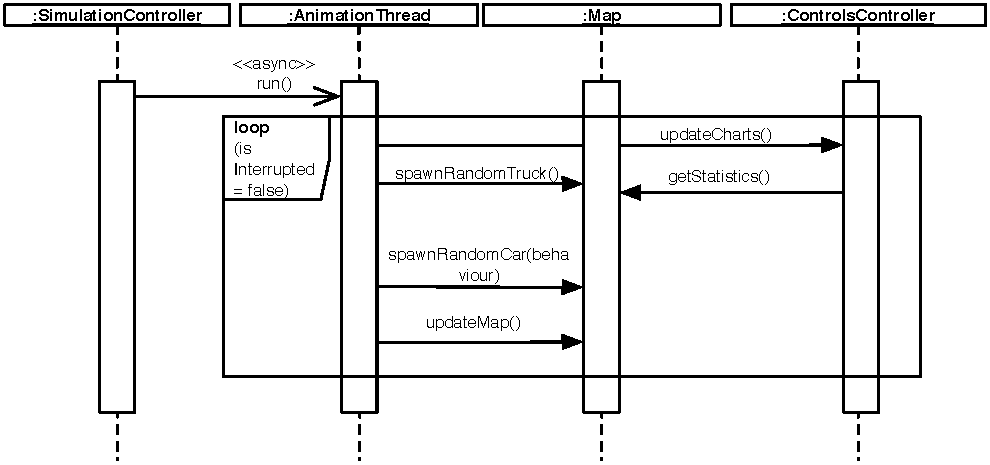
\includegraphics[width=\textwidth]{img/SD_animThread.pdf}
		\caption[Sequence Diagram of the Animation Thread]{Sequence Diagram of the Animation Thread}
		\label{fig:animthread}
	\end{center}
\end{figure}

With the multithreaded execution described above came concurrency related issues. The class Map contains a list to all vehicles currently present in the simulation. Whenever a vehicle is leaving the map, it notifies the SimulationController, which in turn removes the vehicle from the simulation. As the map's \textit{updateMap()} is constantly iterating through its list of vehicles, removing a vehicle from anywhere else than within this loop results in concurrency exceptions.

\begin{wrapfigure}{r}{0.45\textwidth}
	\begin{minipage}{0.45\textwidth}
		\begin{lstlisting}[caption={Car Removal}, label={lst:carRem}]
if(toBeRemoved.contains(v)){
	iter.remove();
	toBeRemoved.remove(v);
	continue;
}	
		\end{lstlisting}
	\end{minipage}
\end{wrapfigure}

In order to overcome this issue we considered both the traditional reader-writer-locking as well as the more advanced read-copy-update pattern, but eventually come to the conclusion but using either of them will introduce an additional scheduling (and implementation) overhead and hence only yield imperceptible performance improvements over the solution we employed (listing~\ref{lst:carRem}). As mentioned earlier, the \textit{updateMap()} method loops through all existing vehicles with each tick, we create a list of vehicles that are about to move the map within the next tick. As soon as the iterator (\textit{iter}) points to a vehicle \textit{v} that is on the \textit{toBeRemoved} list, it is removed and the loop skips one iteration.  

In order to ease the communication between model classes and the \textit{SimulationController} as well as the application classes \textit{MainApp} and \textit{EditorApp} we faced a design decision between the traditional observer pattern and the singleton pattern that allows static access to the required instances. We decided in favour of the singleton pattern, because the situations in which the model communicates with the \textit{SimulationController} are manifold and access to the singleton instance allows for fairly simple communication flows.

\subsection{Testing}
In order to meet all the requirements specified at the beginning of the project, testing forms an integral part in this process. Within the Agile development framework, we felt that Feature Driven Development (FDD) is most adaptable process suited for this project. Hence we decided to test the codes iteratively at the end of each development cycle. We foresaw that writing testing code in a concurrent fashion with the development team may not be an effective way, given the fact that the testing codes may not be working for the final product as incremental changes were made throughout the development. Therefore peer reviews were conducted at early stage to ensure  code quality is kept to standard, that is, each method should be written explicitly to address the problem that needs to be solved. In such manner, we can be assured of a rigid foundation (i.e. the software model) before we even attempt to adding more complicated features.

As the software becomes mature, unit tests were added to the project. We conducted unit testing in JUnit with the support of JemmyFX and ScenicView. JemmyFX is a third party library for testing JavaFX application. It is a test harness which allows the user to simulate user input, i.e. click buttons, entering data. In particular, JemmyFX defines how to get a list of scenes, nodes items, and get text of a \textit{javafx.scene.control.Label} (listing~\ref{lst:checkBox}). We have mainly used this for UI testing. 


\begin{minipage}{0.9\textwidth}
	\begin{lstlisting}[caption={Use JemmyFX syntax to find a checkBox element}, label={lst:checkBox}]

//Identifying the input checkBox element exist
assertEquals(CheckBox.class, new LabeledDock(scene.asParent(), checkBoxName, StringComparePolicy.EXACT).wrap().getControl().getClass());

//Find the label of the checkBox 
LabeledDock cb = new LabeledDock(scene.asParent(), checkBoxName, StringComparePolicy.EXACT);

	\end{lstlisting}
\end{minipage}

Using ScenicView helped us to understand what the UI was built from, allowing us and any other future developers to quickly and efficiently query the properties of a particular element, i.e. finding the properties of a JavaFX button (fig.~\ref{fig:scenicview}). ScenicView provides a tree structure and highlights the item upon it is selected. In the case of unable identifying an elements within the source code, this has been particularly helpful.  
\begin{figure}[h]
	\begin{center}
		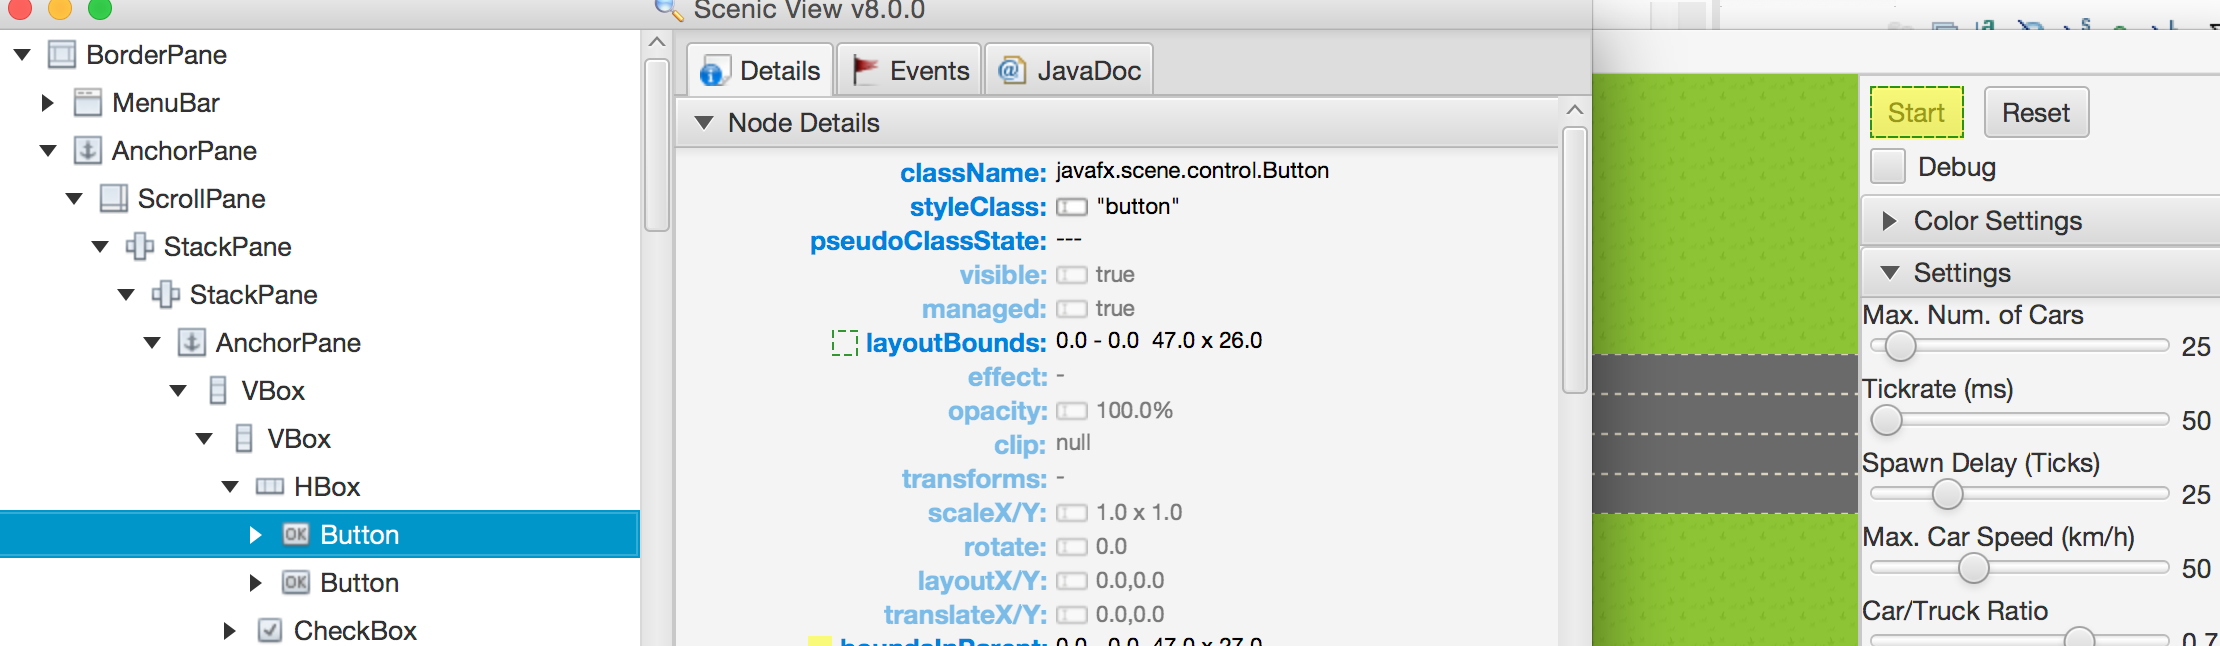
\includegraphics[width=\textwidth]{img/scenicView.png}
		\caption[Identifying properties of Start button with ScenicView]{Identifying properties of Start button with ScenicView}
		\label{fig:scenicview}
	\end{center}
\end{figure}

Since we were trying to achieve a multithreaded application, we reached a point where it was impossible to test every functionality due to the level of nesting and threading was too deep for us to comprehend. Therefore we focused our unit testing mainly on major components (i.e. vehicles, map and the model), in order to ensure features within them work correctly - in return that the application would behave accordingly. With such approach, this gives us the confidence that our code works as we expect it to work. 

It is arguably that there were lots of areas need to be tested. From one perspective, one could argue that the number of test cases could be used as an indication on the software quality. But we believed that unit testing is not about finding bugs. It is to prove that all the components could work together as a whole.  With this mentality, we carried out tests to ensure that the foundation of our code is dependable - at least within the scope of what this project aims to achieve.  

We wrote our test cases in an automated fashion. This allowed us to reduce the workload on manual testing.  A log was produced at the end for every test scenario. This also allowed us to identify problems should each scenario fails. An illustration is shown in fig.~\ref{fig:testCase}. 

\begin{figure}[h]
	\begin{center}
		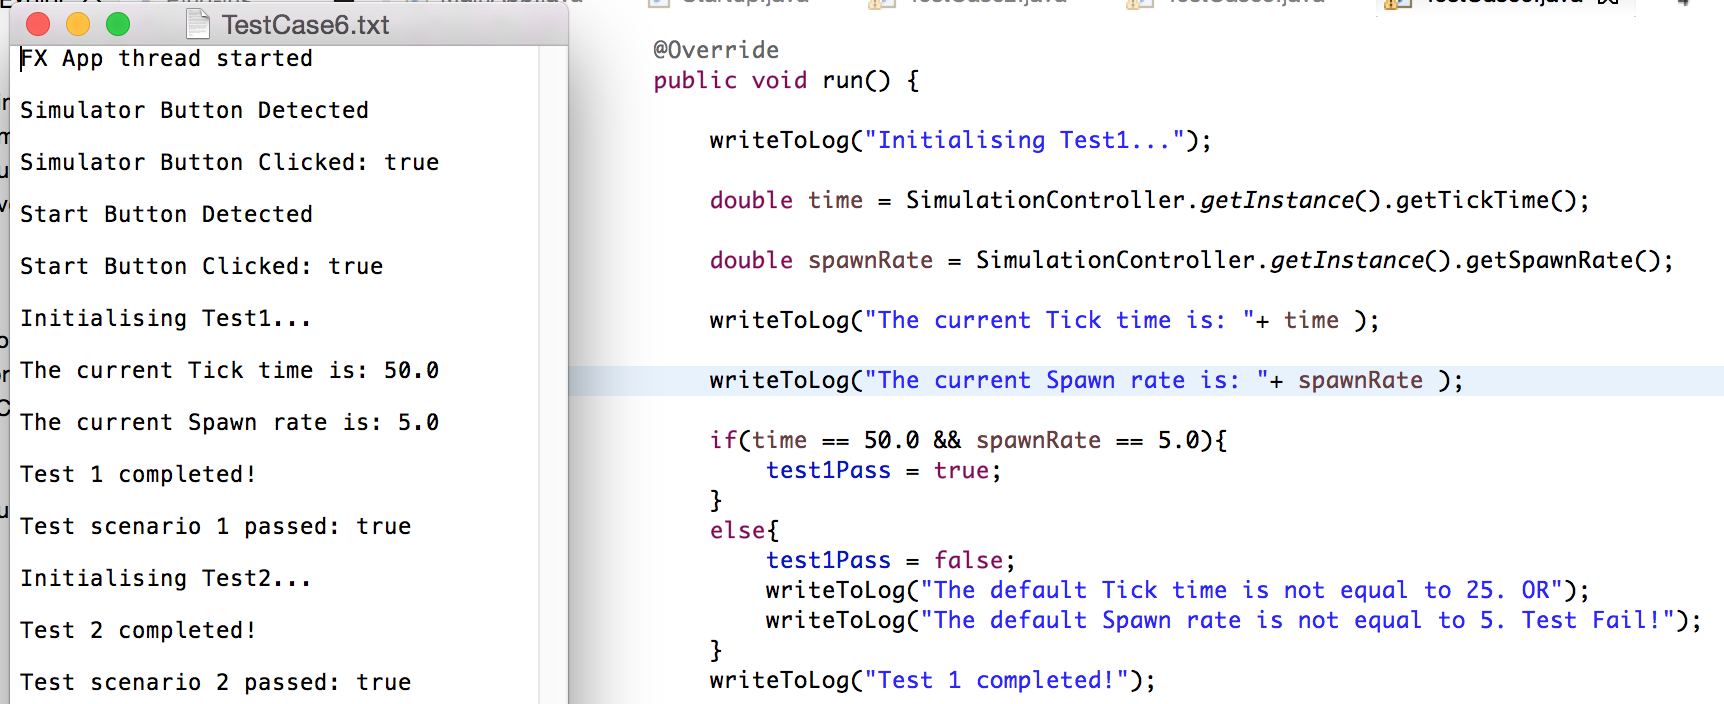
\includegraphics[width=\textwidth]{img/testCase.png}
		\caption{A log is produced after a test execution}
		\label{fig:testCase}
	\end{center}
\end{figure}

In addition, we also looked at the organisation of our code base to further assess the code quality of our software.  To do so we used a commercial tool to analyse the architecture. We produced diagrams such architectural dependencies, heat maps, UML Class Diagrams, as well as metric reports to give us a visual cue on the software internally. We then feed back the analysis to the development team in order to make changes accordingly. For instance, the heat map gave an indication on the level of \textit{lineCount} against \textit{maxCyclomaticComplexity}, as shown in fig.~\ref{fig:heatmap}. The bigger the shape it is the more lines of codes there have been written for a class. The colour depth of a shape indicates the density of its max complexity. At one stage, we identified the \textit{maxCyclomaticComplexity} for the \textit{Car.class} is 58, we were able to reduce it to 21 for the final version.     

\begin{figure}[h]
\begin{minipage}{\textwidth}
	\begin{center}
			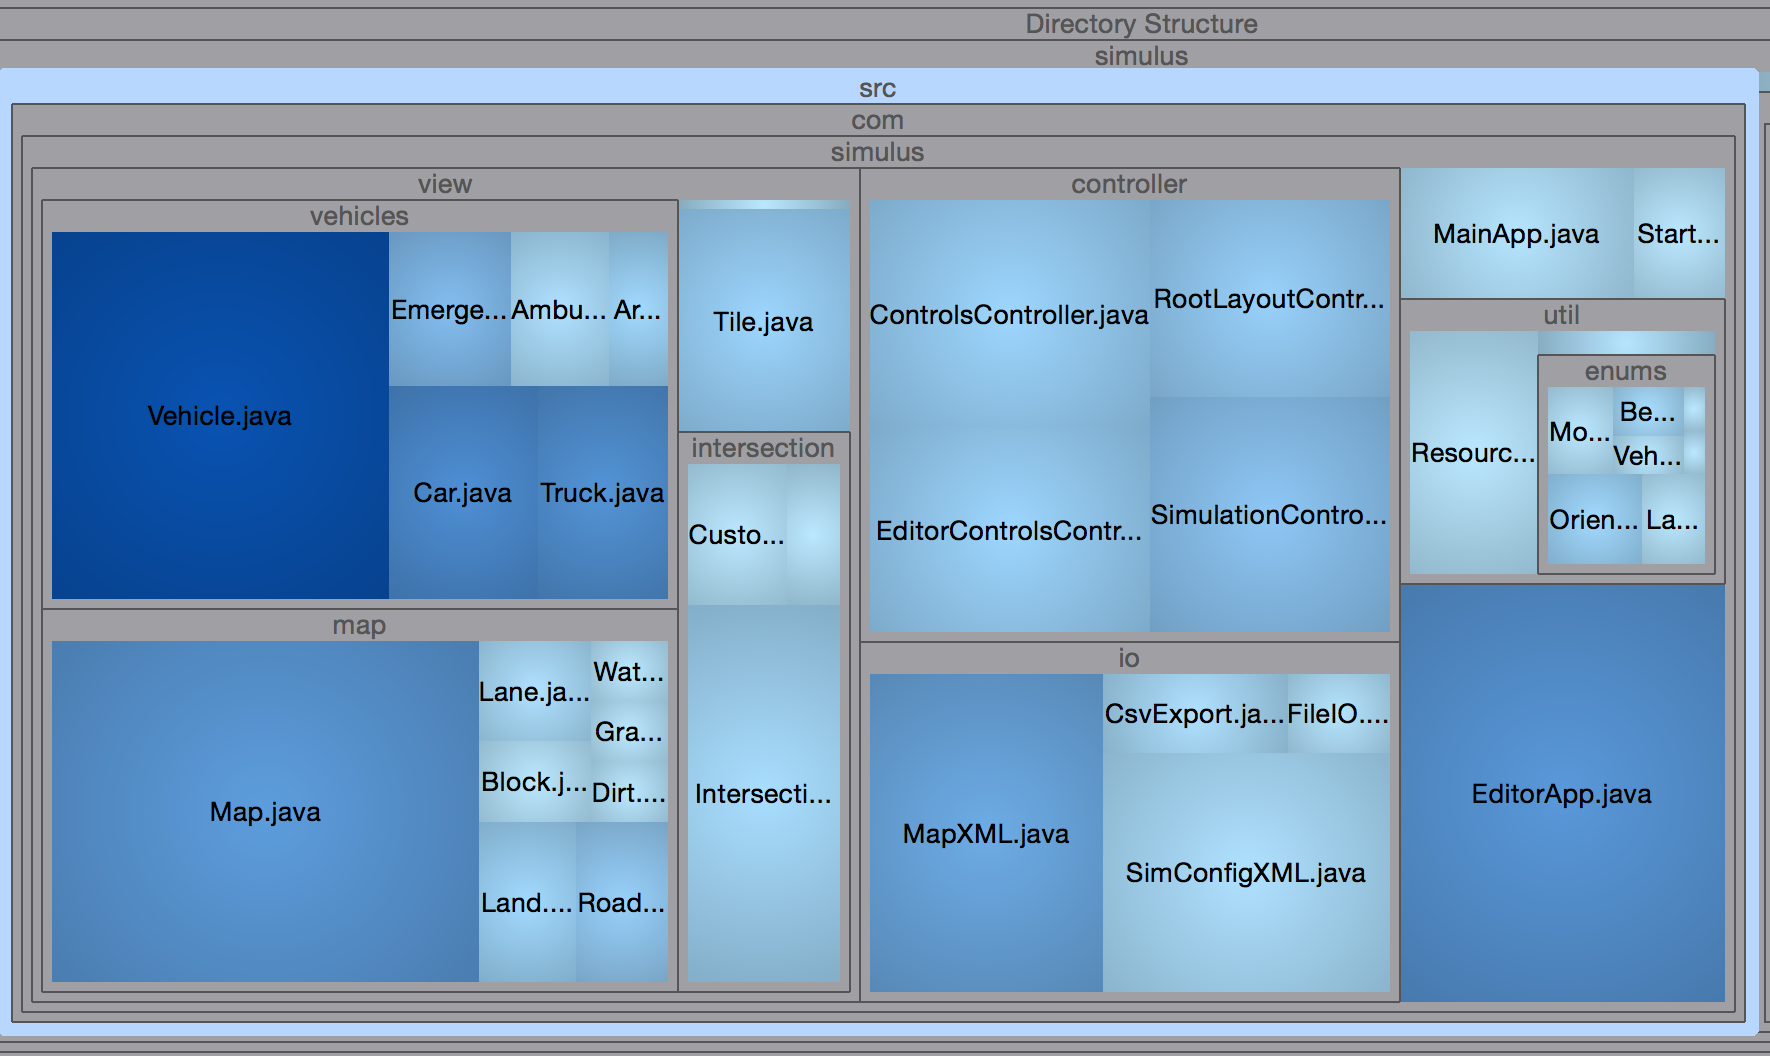
\includegraphics[width=71mm,keepaspectratio ]{img/heatmap.png}
		\caption{Heat Map for the final version of the software}
		\label{fig:heatmap}
	\end{center}
	\end{minipage}
\end{figure}

Fig.~\ref{fig:archIntDependency} illustrated the architectural dependency for our final product. We were assured that the outcome echoed to the requirement and design, though only a small portion of bi-directional calls were made internally. In most case, the architecture is preserved with uni-flow calls. There was no cluster found overall in this project, the architecture can be described more or less as clean, as shown in the figure. 

\begin{figure}[h]
	\begin{center}
			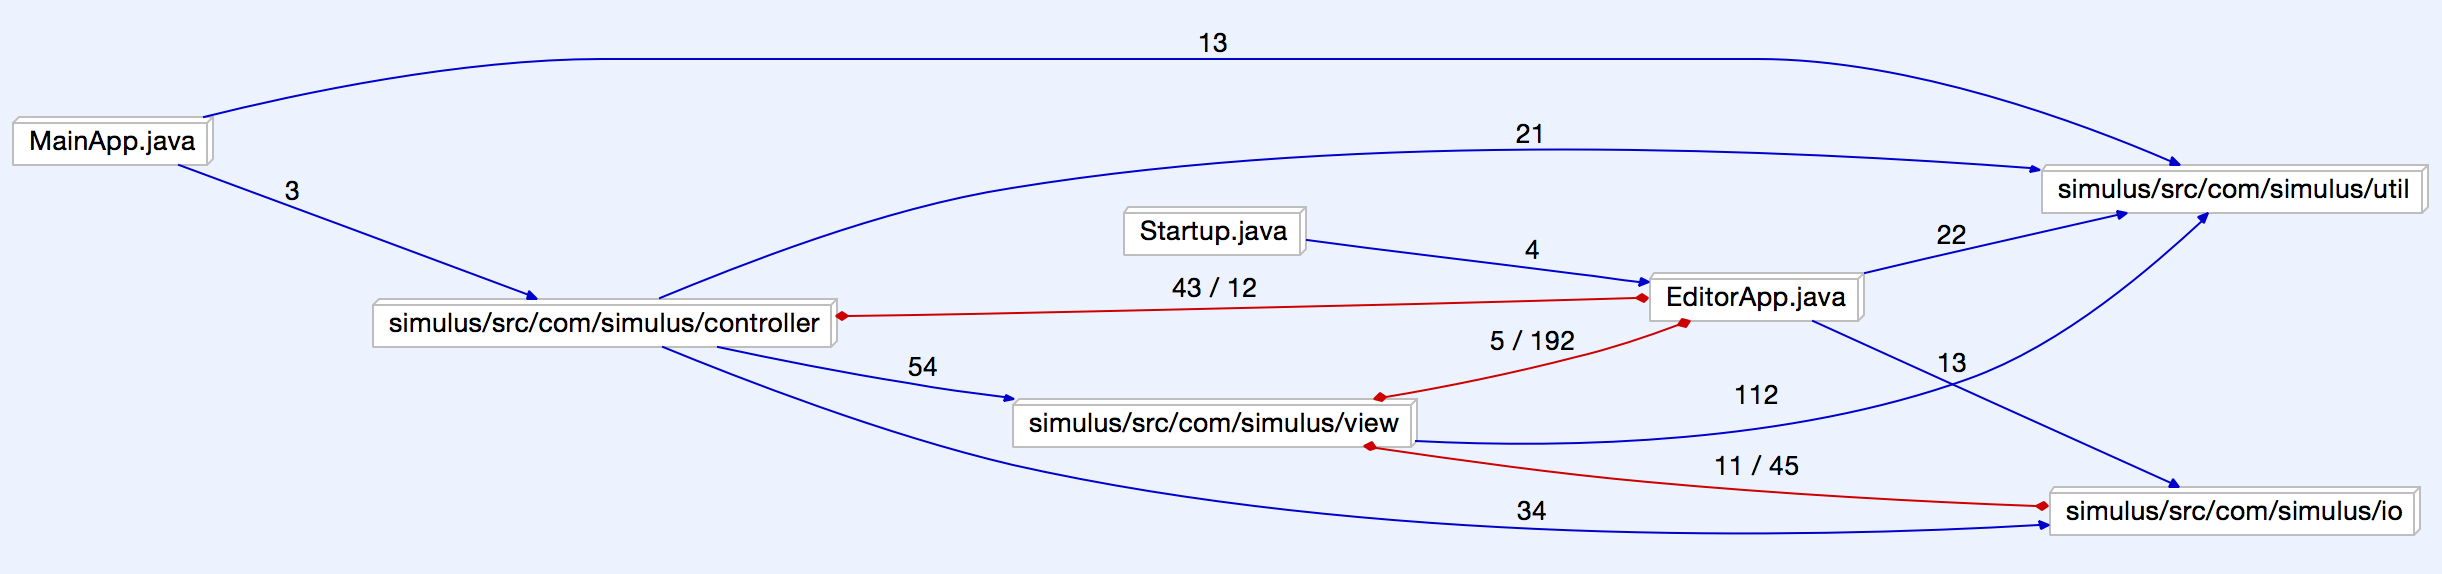
\includegraphics[width=\textwidth]{img/archIntDependency.png}
		\caption{Architecture Internal Dependency}
		\label{fig:archIntDependency}
	\end{center}
\end{figure}

\section{Map Editor}

\subsection{Graphical User Interface}
The majority of the effort with the editor application was on user interaction (UI) design and implementation. Recall the requirements from \ref{ss:req-editor} particularity those for usability (2.1-2.13). Fig.~\ref{fig:finalMapEditor} shows the resulting design chosen which the team felt had met the requirements in whole and one we hope is apparent when using the application to create a map.


\begin{figure}[h]
	\begin{center}
			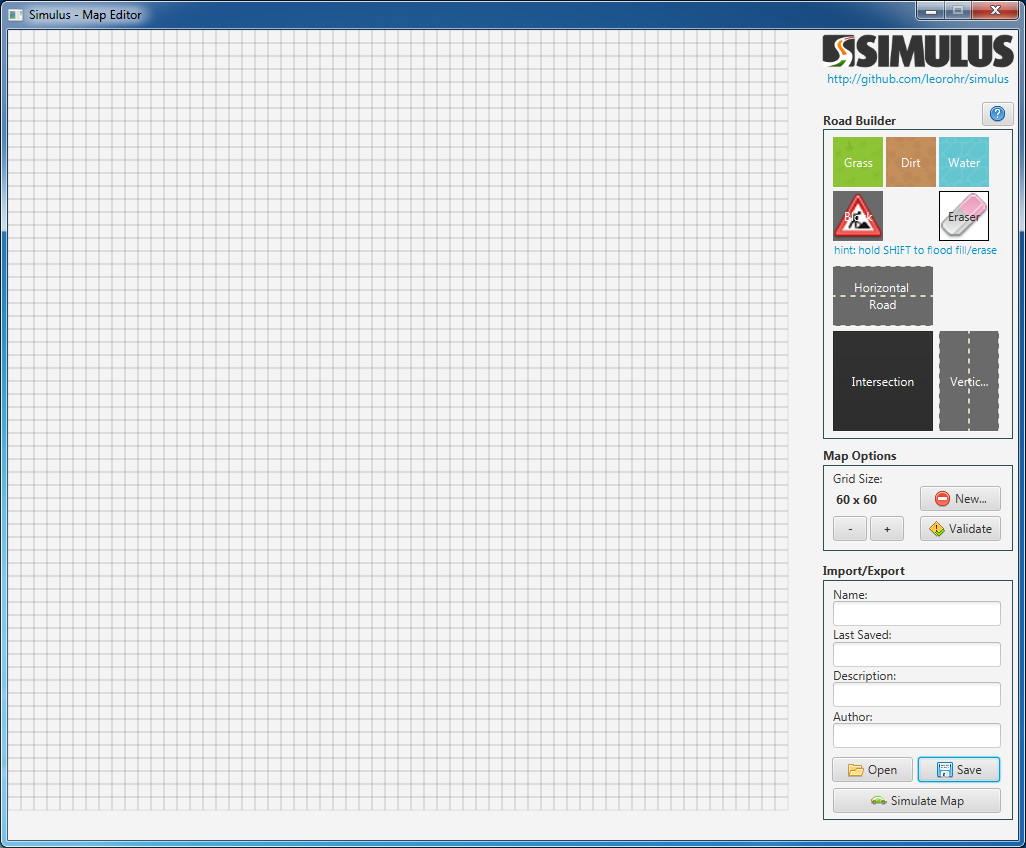
\includegraphics[scale=0.45]{img/mapEditorFinal.png}
		\caption{Resulting map editor design}
		\label{fig:finalMapEditor}
	\end{center}
\end{figure}

\subsection{Flood Fill}
The basis of any map editor is the ability to tag defined areas of desktop real-estate representing a real world instance e.g. land mass. We began by constructing an X*Y cell grid, where X and Y are the number of cells horizontally and vertically and where X=Y. The smallest instance of a map was to be a 40x40 grid yielding 1,600 tiles each needing to be individually tagged. Clearly it was not realistic to expect the user to tag each cell individually. Even when removing the number of tiles that would be tagged using the road and intersection tools, large swathes of the map are left unfilled.  
A method was required that would not only fill the remaining tiles with the users choice of texture but do so intelligently. That is only fill empty cells within in a certain boundary so as not replace existing ones.  This is is better known as a flood fill algorithm and is listed as requirement 2.7 and 2.8 of section \ref{ss:reqs}

There are several techniques for implementing flood fill (cite) of which the 4-way stack based implementation is seen as the simplest and most elegant approach due to its Depth First Search (DFS) recursive property.  The appropriate psudocode is as follows:

% probably need a new listing for psudocode?
\begin{minipage}{0.9\textwidth}
	\begin{lstlisting}[caption={4-way stack based recursive flood fill}, label={lst:stackFloodFill}]
Flood-fill (node, target-tile, replacement-tile):
1. If target-tile is equal to replacement-tile, return.
2. If the tile of node is not equal to target-tile, return.
3. Set the tile of node to replacement-tile.
4. Flood-fill (west of node, target-tile, replacement-tile).
   Flood-fill (east of node, target-tile, replacement-tile).
   Flood-fill (north of node, target-tile, replacement-tile).
   Flood-fill (south of node, target-tile, replacement-tile).
5. Return.
	\end{lstlisting}
\end{minipage}

This procedure was extended with bounds checking in our multidimensional array to give the observable results.

\begin{figure}[h]
	\begin{center}
		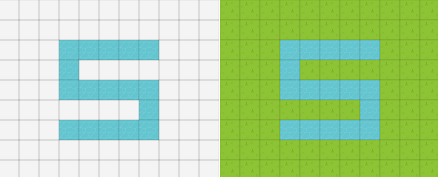
\includegraphics[scale=0.8]{img/floodFill.png}
		\caption[Flood Fill]{Before and after the use of flood fill}
		\label{fig:animthread}
	\end{center}
\end{figure}

Upon initial testing (ref. jerry's editor testing) the recursive approach performed exactly as expected with no functional issues  to report.  However, when the possibility of larger grid sizes was suggested, further testing revealed a fundamental flaw in this approach.  It was found that for a grid size larger than 65x65, a stack overflow would occur thus only partially filling the grid and causing the application to no longer respond.  With the ability to alter grid sizes implemented in later reversions of the simulator and editor applications, further investigation was warranted.

Approaching the literature, the stack over flow observation was commonly experienced and almost expected when using the recursive approach.  Mukherjee and Jana (2010, p.275) state:

 \begin{quotation}
A quick glance on the recursive variant of FloodFill function reveals that the recursive function makes four calls to itself at each step (for 4N connected region). Stack Overflow is the most common exception encountered while dealing with the recursive programs. Each time we call a function recursively, the function parameters, local variables and the return address of code (where to return when we are done with the recursion) are pushed to the stack. If the recursion is too deep, there may be overflowing of stack, where from there is no recovery.
 \end{quotation}
 
Possibly the simplest but least favoured approach was to alter the JVM's configuration parameters and increase the memory reserved for the stack.  Although this would be the simplest 'fix' it was not seen as a suitable solution given the many hardware and JVM configurations and further still, it was not a solution to the fundamental problem.

In the end the the recursive approach was deprecated while a 4-way queue based approach was implemented.  In contrast to the recursive implementation the queue based method is Breadth First Search (BFS) and uses a queue to store each new encountered tile.  The addition of two checks:

\begin{itemize}
  \item if the adjacent tile in question has not been already visited and
  \item if the tile is not of the target type
\end{itemize}

allowed for a tile to be added to the queue, replaced and dequeued in subsequent iterations. The relevant psudocode for the queue based approach is:

% probably need a new listing for psudocode?
\begin{minipage}{0.9\textwidth}
	\begin{lstlisting}[caption={4-way queue based flood fill}, label={lst:queueFloodFill}]
Flood-fill (node, target-tile, replacement-tile):
 1. If target-tile is equal to replacement-tile, return.
 2. Set Q to the empty queue.
 3. Add node to the end of Q.
 4. While Q is not empty: 
 5.     Set n equal to the last element of Q.
 6.     Remove last element from Q.
 7.     If the tile of n is equal to target-tile:
 8.         Set the tile of n to replacement-tile and mark 
 9			"n" as processed.
 10.        Add west node to end of Q if not yet processed.
 11.        Add east node to end of Q if not yet processed.
 12.        Add north node to end of Q if not yet processed.
 13.        Add south node to end of Q if not yet processed.
 14. Return.
	\end{lstlisting}
\end{minipage}

With this new revised function, grid size was no longer an issue and a flood fill of an empty 200x200 grid (larger than any suggested grid size) completed successfully without any noticeable delay.
\paragraph{}
To ensure the new approach would be indeed suitable for the set grid sizes, some simple measurements were taken.  The two algorithms were used to fill an empty grid with a 'grass' land tile, repeated three times and an average calculated.  The results shown in fig.\ref{fig:floodChart} clearly show that although the recursive stack based implementation performs on average 70\% faster, it was unable to function for grid widths greater than 60 in our set.  Although this may seem wholly a failure for the queue based implementation, it is important to point out that this equates to ~10ms difference. Not noticeable by any human operator.  Even more interesting was that the results quoted were based on First Time Run (FTR) values, immediately after launching the editor. Using the same two routines on subsequent occasions would yield repeated values as low as 10-16ms per fill.
 
\begin{figure}[h]
\centering
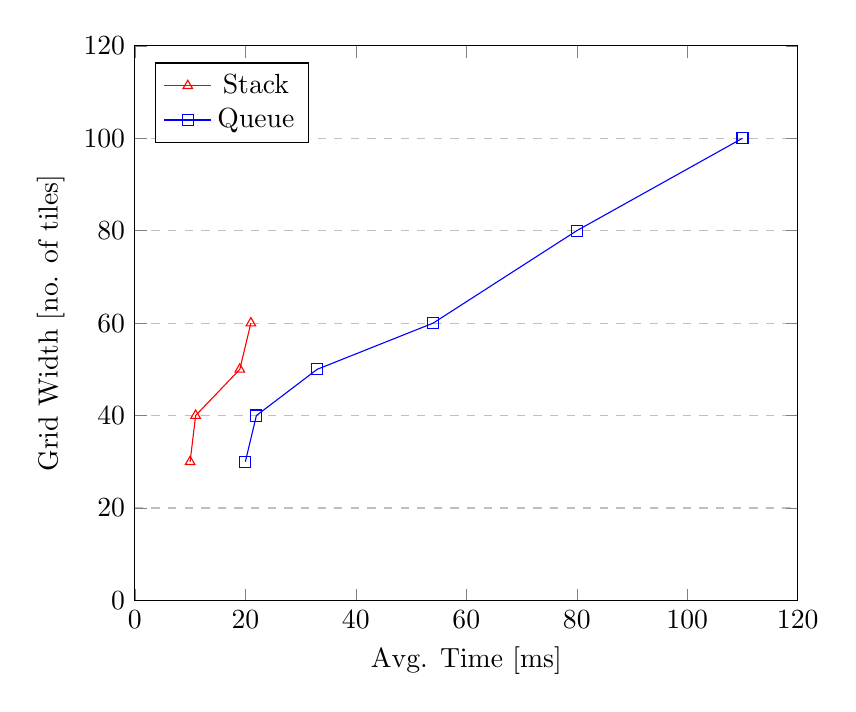
\begin{tikzpicture}
\begin{axis}[
    xlabel={Avg. Time [ms]},
    ylabel={Grid Width [no. of tiles]},
    xmin=0, xmax=120,
    ymin=0, ymax=120,
    xtick={0,20,40,60,80,100,120},
    ytick={0,20,40,60,80,100,120},
    legend pos=north west,
    ymajorgrids=true,
    grid style=dashed,
]
\addplot[
    color=red,
    mark=triangle,
    ]
    coordinates {
    (10,30)(11,40)(19,50)(21,60)
    };
\addplot[
    color=blue,
    mark=square,
    ]
    coordinates {
    (20,30)(22,40)(33,50)(54,60)(80,80)(110,100)
    };
    \legend{Stack, Queue}
\end{axis}
\end{tikzpicture}
\caption{Average execution time for flood fill}
\label{fig:floodChart}
\end{figure}

It must be noted that the new method is no longer as concise as a definition compared to the original but it was a subtle sacrifice for the benefits it yielded.
	\section{Team Work}
\label{sec:team_work}
Critical to the success of our project has been our ability to work as a collective with a clear objective, translated into practise by our organisation, use of tools and overcoming challenges when posed. We now focus on some of these aspects.

\subsection{Development Process}
As outlined in the initial report, we selected to follow an Iterative and Incremental Development (IID) process. This was evident in the group's Gantt chart (ref appendix) having planned short development cycles. These cycles comprised of a requirements and planning task to identify what was to be achieved and how it was to be accomplished. We then progressed to possible design solutions that would meet the requirements. We developed the feature and then carried out testing against it. Collectively evaluating the feature and our efforts in that week was the final stage of a cycle. Each feature had an exit point, where once the requirements where met, we could progress. In order to establish the priority for each feature and thus the order in which it would be implemented, the perceived value gained by each was our indicator wholly based on the MoSCoW analysis, carried out in section \ref{sec:reqs}.

A notable benefit of the above approach was that it encouraged modular design, facilitating deconstruction of large, undefined requirements into manageable features: "Map drawing feature" was refined to "land tiles have three different instances; grass, dirt and water" and "simulator has export button" to "there is the ability to export simulation parameters from within the simulator", etc.  
Probably the most beneficial aspect was that we were able to ascertain our development progress early on and thus adjust the time dedicated to the project, manoeuvring group members where additional effort was required. The iterative feedback not only allowed us to evaluate the software we were developing but our own techniques and group dynamics on a weekly basis.

\subsection{Team Policy}
The team's identified approach to management was wholly democratic opting to vote on most points of contention, from the triviality of tile colours to the more pressing decision of using a continuous model over the discrete prototype.

\begin{lstlisting}[caption={Decision Making Agreement}]
* Each individual has the opportunity to voice their concerns
* Each individual has an equal vote on an issue
* The majority vote is the deciding vote
\end{lstlisting}
 
Although one may have concern that this policy could lead to inaction, we found that system worked well for us on this occasion.  Perhaps this was in part due to the individual members, their personalities and working mentality. We had minimal, if any, conflicts to resolve, as a result of open discussion and brainstorming within the allocated weekly meetings and Facebook group.

\subsection{GitHub}
Our tool set for collaboration may seem inadequate at first glance, listing Facebook, WhatsApp and GitHub only. Upon closer inspection it is immediate that we fully embraced GitHub and most of it's available features. We have found GitHub to be an accomplished tool for software projects and can fully appreciate why it is popular in industry and open-source projects. For several of us, it was our first exposure to distributed version control and source code management but we can be confident that all facets of our group work was enhanced by the use of this tool.

The team's usage of GitHub was immediate but was largely adopted once we had made the decision to change to a continuous model.  Whereas previously we had worked in a single branch, we created an additional two - a 'model' and 'editor' for each area of the project.  This allowed the two development sub teams to work independently. At strategic points and at the end of a development cycle \ref{subsec:Development Process}, we would aim to merge the two branches with the necessary members present. As useful was the 'issues' feature where any individual may create a task for himself or for the team as a whole. We were able to translate functional requirements, to almost atomic levels in some cases, and assign them to team members. The ability to post questions and comments against an issue was helpful and the tagging feature became a handy method to quickly prioritise tasks. The team  did attempt to create suitable Wiki pages for the project but this was not entirely accomplished as expanded on in the next section.

\subsection{Challenges}
Inevitably we did face some challenges, none that were detrimental to the overall completion and achievement of our aims. However the basis of learning from our experience is that we are clear on what these were and how it was overcome. 

Having praised the value of using a Git repository in section \ref{subsec:GitHub}, it is important to understand that good communication is still paramount when working through such a system. Not being clear of the current classes a colleague is working on led to us on one occasion suffering a delay when a commit was made without reviewing the conflicts. Increased communication, through private messaging and the GitHub issues feature, meant this was no longer an issue once identified. All members made others aware of their current activity, progress and subsequent tasks to be tackled.

The team felt additional informational pages should have been posted to our Git's Wiki. An effort was made initially but not sufficiently to fully document the project. Unfortunately we were unable to find the time to make this a reality but it would be feasible to complete at a later date.

\todo refer to github (meeting minutes)

	\section{Evaluation}
\label{ss:eval_sim}
In terms of the realisation of initially set requirements, we were able to meet them all except for the inclusion of external map sources (requirement 3b in section~\ref{sec:reqs}). This, however, was associated with the "could have" priority class and hence is an acceptable shortcoming. As our map model is based on fixed sized tiles, it would require intense translation to reproduce a map from sources like Google Maps or KML files due to their high resolution. 

As described in section \ref{subsec:design}, we began using a discrete space model and changed to a continuous model later on. This change was a product of improved thinking, as we realised that the restrictions imposed by a discrete space representation outweigh the benefits of the easier implementation that comes with it.

At the beginning of the project we implemented a model-view-controller pattern. However, during the course of the implementation it became apparent, that strictly following this pattern is impractical for this particular project. In the current state of the software, the initially separated model and view are combined in the view package. An example for this consolidation are the vehicle classes. They extend the JavaFX class \textit{Rectangle}, which is used to visualise the different types of vehicles. Nonetheless, vehicles do also know their position in the map model and compute their movement on their own - both functionality that belongs to the model in a strict MVC architecture.

The methods that compute vehicle movements require numerous of checks for the vehicle's environment. An example would be the method by which a car overtakes another. Multiple tiles of the adjacent lane must first be checked for the conditions to be met for this manoeuvre to take place. The exact tiles that need to be checked currently depend on the direction of the vehicles' movement and hence these checks come with a lot of nested conditional statements. The \textit{attemptOvertake} method in the \textit{Vehicle} class exhibits a cyclomatic complexity of 34, therewith being the most complex method in our source code (see fig.~\ref{fig:heatmap}). Reducing the complexity for this method along with others would most likely improve the scaling of simulator performance with a higher number of vehicles. Implementing these changes would require a major redesign of the simulation logic and was hence deemed as infeasible to do within the short duration of this project.

Maps are persisted using the XML. Each map-file contains data for every single tile on the map. Unfortunately, the XML specification we used does not specify the grouping of tiles to an intersection, forcing us to recreate the intersections as soon as an intersection tile is encountered while reading the map. This means that the algorithm will create an intersection at the encountered tile and hence create the tiles 3 columns to the right and 3 rows down without reading any further tile information from the XML file. To ensure that intersections are created correctly, we have to create a 2D boolean array the size of the map (i.e. 40x40, 60x60 or 80x80) to keep track of tiles that have been loaded successfully. 

Our model currently only supports roads with four lanes and dual carriageways. As adding support for different lane models and road sizes will increase the capabilities and functionality of both simulator and editor, we consider this a suitable task for further development of the software. 

All five group members were involved in the creation of the code. Collaboration and communication was eased through extensive use of the Git Issues feature to track problems and progress in solving them (cf. section~\ref{sec:team_work}). Working in separate branches of the repository when working on the same files or related behaviour allowed every team member to contribute to the codebase continuously.  

\subsection{Future Work}
%evaluation of editor?

	\section{Peer Assessment}

	\fancyfoot[C]{\thepage}
	\bibliographystyle{plain}
	\bibliography{literature}
	
	\appendix
	\chapter{Gitlog}
\begin{center}
\begin{longtabu} to \textwidth {|
    X[4,l]|
    X[3,c]|
    X[8,l]|}
    \hline
    \textbf{Author} & \textbf{Date} & \textbf{Message} \\ \hline
leorohr & 2015-01-15 & init \\ \hline
leorohr & 2015-01-15 & Exclude mac-specific .DS\_Store file \\ \hline
leorohr & 2015-01-25 & initial project setup .txt files in mode, view, controller package can be removed, as soon as classes are added. \\ \hline
ebrahim & 2015-01-29 & Moving a car across the screen \\ \hline
Alan & 2015-01-29 & Creating documents folders and files \\ \hline
leorohr & 2015-01-30 & First UI Draft \\ \hline
ebrahimmalek & 2015-01-30 & A node moving across a scene \\ \hline
leorohr & 2015-01-30 & Initialise MainApp \\ \hline
ebrahimmalek & 2015-01-30 & Merge branch `master' of https://github.com/leorohr/simulus.git \\ \hline
ebrahimmalek & 2015-01-30 & Initial Vehicle and Car objects. \\ \hline
leorohr & 2015-01-30 & First draft of the overall mode. ModelTester is a class purely for development purposes and will be removed later. Map contains the main logic and represents the Grid cars move on. \\ \hline
leorohr & 2015-01-30 & Small correction and added printGrid method \\ \hline
ebrahimmalek & 2015-01-30 & Merge branch `master' of https://github.com/leorohr/simulus.git \\ \hline
leorohr & 2015-01-31 & Small tweaks and bug fixes. ModelTester does now spawn up to 4 cars in the entrypoints but stops then, since the cars are not moving anywhere yet. \\ \hline
Alan & 2015-02-01 & Gantt Chart v2 \\ \hline
Alan & 2015-02-01 & Gantt Chart v3 \\ \hline
Alan & 2015-02-01 & Gantt Chart File for Wiki \\ \hline
jerry & 2015-02-03 & Changed/Added directories \\ \hline
jerry & 2015-02-03 & Major remodelling multi lane/road \\ \hline
Alan & 2015-02-03 & Draft - Initial Report Section 2 r01 \\ \hline
Alan & 2015-02-03 & Gantt Chart r03 \\ \hline
Alan & 2015-02-03 & Draft - Initial Report Section 2 r01 Source File \\ \hline
ebrahimmalek & 2015-02-03 & Merge branch `master' of https://github.com/leorohr/simulus.git \\ \hline
ebrahimmalek & 2015-02-03 & Our cars can now move in all specified directions on demand. \\ \hline
leorohr & 2015-02-04 & Added class diagram for the model package \\ \hline
leorohr & 2015-02-04 & Merge branch `master' of https://github.com/leorohr/simulus.git \\ \hline
ebrahimmalek & 2015-02-04 & Added traffic lights. They change using a thread with an endless loop. They are cool. \\ \hline
Alan & 2015-02-04 & Gantt Chart r04 \\ \hline
ebrahimmalek & 2015-02-04 & Traffic Lights that change using an endless loop within a thread. \\ \hline
ebrahimmalek & 2015-02-04 & Merge branch `master' of https://github.com/leorohr/simulus.git \\ \hline
leorohr & 2015-02-05 & Moved enumerations to com.simulus.util.enums \\ \hline
leorohr & 2015-02-05 & Merge branch `master' of https://github.com/leorohr/simulus.git \\ \hline
leorohr & 2015-02-05 & Implemented MapUpdateListener that listens to changes in the current state of the map (refers to issue \#4) \\ \hline
leorohr & 2015-02-05 & Added SimulationController, which is in charge of the main simulation supervision Mapped Start and Stop button to the controller's methods (refers to \#12) \\ \hline
leorohr & 2015-02-05 & Map now exhibits the singleton-pattern to make it accessible for controllers. The map's size default is set to 10x10, but can be assigned by calling Map.setSize(int). closes \#4 \\ \hline
leorohr & 2015-02-05 & small bugfix \\ \hline
leorohr & 2015-02-05 & Updated class diagram \\ \hline
leorohr & 2015-02-05 & forgot to actually add the controller to list of listeners \\ \hline
leorohr & 2015-02-05 & Changed variable name from ambigious `map' to `grid' \\ \hline
Alan & 2015-02-05 & Draft - Initial Report Section 2 r02 \\ \hline
ebrahimmalek & 2015-02-06 & Merge branch `master' of https://github.com/leorohr/simulus.git \\ \hline
jerry & 2015-02-06 & Major modification to the package com.simulus.model \\ \hline
jerry & 2015-02-06 & Merge branch `master' of https://github.com/leorohr/simulus.git \\ \hline
leorohr & 2015-02-06 & removed merge conflict descriptions \\ \hline
leorohr & 2015-02-06 & Added notifySpawnCar(..) to the mapupdatelistener \\ \hline
leorohr & 2015-02-06 & Moved Light-enum to enum package \\ \hline
ebrahimmalek & 2015-02-06 & New look on lights. getInstance() method on MainApp \\ \hline
ebrahimmalek & 2015-02-06 & Merge branch `master' of https://github.com/leorohr/simulus.git \\ \hline
leorohr & 2015-02-06 & passing gridsize to app \\ \hline
leorohr & 2015-02-06 & Now allows navigation from a lane to its enclosing road object. Further navigability (to the road's tile) is not necessary, so far. closes \#6 \\ \hline
leorohr & 2015-02-06 & doc \\ \hline
ebrahimmalek & 2015-02-06 & Report \\ \hline
ebrahimmalek & 2015-02-06 & Report \\ \hline
ebrahimmalek & 2015-02-06 & Ticking in GUI \\ \hline
Alan & 2015-02-06 & Draft - Initial Report Section 1 r01 \\ \hline
leorohr & 2015-02-07 & passing vehicle-list to ui \\ \hline
leorohr & 2015-02-07 & moveForward method \\ \hline
alan-s & 2015-02-07 & Draft - Initial Report All r01 \\ \hline
leorohr & 2015-02-07 & Intersection class Vehicles only move if no vehicle in front and, if facing an intersection, the light is green \\ \hline
leorohr & 2015-02-07 & Merge branch `master' of https://github.com/leorohr/simulus.git \\ \hline
Paul Barella & 2015-02-07 & Collated research \\ \hline
leorohr & 2015-02-07 & checkIntersection() is called now \\ \hline
ebrahimmalek & 2015-02-07 & Roads \\ \hline
ebrahimmalek & 2015-02-07 & Merge branch `master' of https://github.com/leorohr/simulus.git \\ \hline
alan-s & 2015-02-07 & Revision 02 \\ \hline
alan-s & 2015-02-07 & Revision 03 \\ \hline
Paul Barella & 2015-02-07 & Fixed header problem \\ \hline
ebrahimmalek & 2015-02-07 & Renamed classes Added SimulationController functionality Updated moveForward method \\ \hline
ebrahimmalek & 2015-02-07 & Merge branch `master' of https://github.com/leorohr/simulus.git \\ \hline
leorohr & 2015-02-07 & changes \\ \hline
ebrahimmalek & 2015-02-07 & Change \\ \hline
ebrahimmalek & 2015-02-07 & r \\ \hline
ebrahimmalek & 2015-02-07 & Merge branch `master' of https://github.com/leorohr/simulus.git \\ \hline
ebrahimmalek & 2015-02-07 & Moving cars \\ \hline
alan-s & 2015-02-07 & Revision 4 \\ \hline
alan-s & 2015-02-07 & Draft - Initial Report All r05 4 pages :) 1199 words \\ \hline
ebrahimmalek & 2015-02-07 & Cars in correct positions\ldots{} and moving! \\ \hline
ebrahimmalek & 2015-02-07 & Merge branch `master' of https://github.com/leorohr/simulus.git \\ \hline
leorohr & 2015-02-07 & require JDK8 \\ \hline
leorohr & 2015-02-07 & Merge branch `master' of https://github.com/leorohr/simulus.git \\ \hline
leorohr & 2015-02-07 & removed updateSpawnedCar \\ \hline
leorohr & 2015-02-07 & fixed out of bounds error \\ \hline
leorohr & 2015-02-07 & cars do disappear correctly now \\ \hline
leorohr & 2015-02-07 & asd \\ \hline
leorohr & 2015-02-07 & switchlights \\ \hline
leorohr & 2015-02-07 & asd \\ \hline
Paul Barella & 2015-02-07 & Kept it clean and simple. As there's a lot of points in our report I've tried to keep it as clear as possible but while still giving prompts in case we forget what we're supposed to talk about. Any comments or suggestions? \\ \hline
leorohr & 2015-02-07 & few typos \\ \hline
leorohr & 2015-02-07 & few typos \\ \hline
leorohr & 2015-02-07 & Intersection can now inform the map when the lights are switched \\ \hline
leorohr & 2015-02-07 & Map is now drawn on call from SimulationController and based on the map stored in the model \\ \hline
leorohr & 2015-02-07 & Cool map, cool simulation \\ \hline
leorohr & 2015-02-07 & more, faster, better \\ \hline
leorohr & 2015-02-07 & synchronized exception \\ \hline
leorohr & 2015-02-07 & removed main method from FXMovingCar to avoid confusion \\ \hline
leorohr & 2015-02-07 & next attempt to synchronize the VehicleList access \\ \hline
jerry & 2015-02-07 & Added Minutes from previous meeting 06.02.2015 \\ \hline
leorohr & 2015-02-07 & Removed mainView.fxml Added Controls.fxml \\ \hline
leorohr & 2015-02-07 & Merge branch `master' of https://github.com/leorohr/simulus.git \\ \hline
leorohr & 2015-02-07 & removed scenecontroller, irrelevant. \\ \hline
leorohr & 2015-02-08 & updated class diagram for model package \\ \hline
Alan & 2015-02-08 & Draft - Initial Report All r06 \\ \hline
Alan & 2015-02-08 & Draft - Initial Report All r06 \\ \hline
Alan & 2015-02-08 & Latest Gantt Chart r05 and MS Project file \\ \hline
Alan & 2015-02-08 & Latest Gantt Chart r05 Typo \\ \hline
Alan & 2015-02-08 & Initial Presentation in Latex format \\ \hline
Alan & 2015-02-08 & Incorrect slide title in Latex \\ \hline
Paul Barella & 2015-02-08 & Amendments to grammar. Some small changes to grammar etc. \\ \hline
Paul Barella & 2015-02-08 & Powerpoint update Updated Powerpoint presentation to mirror Latex version more closely. \\ \hline
Alan & 2015-02-09 & Initial Report \\ \hline
leorohr & 2015-02-09 & added timetable \\ \hline
leorohr & 2015-02-09 & Intersection now passes itself to controller when its lights switch. Controller then passes that object to UI to allow trafficlight visualisation \\ \hline
jerry & 2015-02-09 & Updated Preivous meeting notes \\ \hline
jerry & 2015-02-09 & Added Simulus Project meeting 09/02/2015 \\ \hline
ebrahimmalek & 2015-02-09 & Intersections created for View. \\ \hline
ebrahimmalek & 2015-02-09 & Merge branch `master' of https://github.com/leorohr/simulus.git \\ \hline
Alan & 2015-02-09 & Initial Report with Table \\ \hline
leorohr & 2015-02-09 & report \\ \hline
ebrahimmalek & 2015-02-09 & Traffic Lights are now visible. model/Road -\textgreater{} now has an ID view/VIntersection -\textgreater{} Receives that ID from the model \\ \hline
ebrahimmalek & 2015-02-09 & Merge branch `master' of https://github.com/leorohr/simulus.git \\ \hline
Alan & 2015-02-09 & Presentation Slide - Gantt \\ \hline
ebrahimmalek & 2015-02-09 & A few grammatical issues (sorry Alan). \\ \hline
ebrahimmalek & 2015-02-09 & Merge branch `master' of https://github.com/leorohr/simulus.git \\ \hline
ebrahimmalek & 2015-02-09 & Stuff that it wants me to push \\ \hline
Alan & 2015-02-09 & Presentation Slide - Table \\ \hline
ebrahimmalek & 2015-02-09 & Concurrent Modification Problem possibly fixed. Ran for 5 minutes. \\ \hline
ebrahimmalek & 2015-02-09 & Merge branch `master' of https://github.com/leorohr/simulus.git \\ \hline
Alan & 2015-02-09 & Presentation Slide - New Screenshot \\ \hline
ebrahimmalek & 2015-02-09 & Now fits on 4 pages \\ \hline
ebrahimmalek & 2015-02-09 & Merge branch `master' of https://github.com/leorohr/simulus.git \\ \hline
leorohr & 2015-02-09 & Uploaded version of the initial report \\ \hline
leorohr & 2015-02-09 & removed logfiles \\ \hline
leorohr & 2015-02-10 & report \\ \hline
Paul Barella & 2015-02-10 & Grammar. Restored previously overwritten updates- using latest submitted version. \\ \hline
leorohr & 2015-02-10 & report \\ \hline
Alan & 2015-02-11 & Latest Presentation \\ \hline
ebrahimmalek & 2015-02-17 & First attempt at a continuous traffic simulator. \\ \hline
ebrahimmalek & 2015-02-17 & Sorry, didn't add the new packages with the last commit. Here they are \\ \hline
leorohr & 2015-02-18 & moved discrete prototype to subfolder \\ \hline
leorohr & 2015-02-18 & merge continuous and master \\ \hline
leorohr & 2015-02-18 & added ui controller classes \\ \hline
leorohr & 2015-02-18 & renamed packages from continuous to simulus \\ \hline
leorohr & 2015-02-18 & added ambulance \\ \hline
leorohr & 2015-02-18 & Removed menuBar as it is not necessary for now. Enabled controls-UI again \\ \hline
leorohr & 2015-02-19 & moved ambulance to view package \\ \hline
leorohr & 2015-02-19 & moved ambulance \\ \hline
leorohr & 2015-02-19 & Renamed VIntersection to Intersection \\ \hline
ebrahimmalek & 2015-02-19 & Lanes Added. Cars will now properly remove off screen regardless of the number of tiles. \\ \hline
ebrahimmalek & 2015-02-19 & Merge branch `master' of https://github.com/leorohr/simulus.git \\ \hline
ebrahimmalek & 2015-02-19 & Merging stuff \\ \hline
leorohr & 2015-02-19 & added getTileSize() \\ \hline
leorohr & 2015-02-19 & Merge branch `master' of https://github.com/leorohr/simulus.git \\ \hline
leorohr & 2015-02-19 & map and stuff \\ \hline
ebrahimmalek & 2015-02-19 & Some Map Additions \\ \hline
ebrahimmalek & 2015-02-19 & Classes not used in editor \\ \hline
ebrahimmalek & 2015-02-19 & Change \\ \hline
ebrahimmalek & 2015-02-19 & Removed some stuff we dont need in editor \\ \hline
ebrahimmalek & 2015-02-19 & Some editor changes \\ \hline
leorohr & 2015-02-19 & stuff \\ \hline
ebrahimmalek & 2015-02-19 & Some changes \\ \hline
ebrahimmalek & 2015-02-19 & Some changes \\ \hline
ebrahimmalek & 2015-02-19 & Ready to start editor \\ \hline
ebrahimmalek & 2015-02-19 & Editor Side Buttons Working \\ \hline
leorohr & 2015-02-19 & a lot of stuff \\ \hline
leorohr & 2015-02-19 & removed pdfs \\ \hline
ebrahimmalek & 2015-02-20 & Adding land works \\ \hline
ebrahimmalek & 2015-02-20 & Stuff \\ \hline
ebrahimmalek & 2015-02-20 & Stuff \\ \hline
ebrahimmalek & 2015-02-20 & Can add intersections, roads and land \\ \hline
paulbarella & 2015-02-20 & Seperated Editor from MainApp Added Road Direction buttons Drag-to-draw implemented (Land and Roads) \\ \hline
Alan & 2015-02-20 & Mapping package consisting of XML Map class with methods for reading from and to an XML map class. Example XML map schema attached. Test class (that can be deleted) to show input/output \\ \hline
Alan & 2015-02-20 & Rename of mapping tile class \\ \hline
leorohr & 2015-02-21 & added paths to intersections \\ \hline
leorohr & 2015-02-21 & reintroduced UI functionality \\ \hline
leorohr & 2015-02-21 & app is not resizable anymore \\ \hline
leorohr & 2015-02-21 & resized grid, 800x800px, 40x40 tiles, hash-like map \\ \hline
leorohr & 2015-02-21 & cars are spawning exactly in the middle of a lane now \\ \hline
ebrahimmalek & 2015-02-21 & Overtaking cars and car behaviors \\ \hline
ebrahimmalek & 2015-02-21 & Behaviors \\ \hline
ebrahimmalek & 2015-02-21 & Merge branch `master' of https://github.com/leorohr/simulus.git \\ \hline
leorohr & 2015-02-21 & added trucks and cartruck-ratio slider \\ \hline
leorohr & 2015-02-24 & Redesign: Moved Simulation execution to SimulationController. For now simulation is run without AnimationTimer, but in a separate thread. Collision detection is working again, however, cars stop randomly in the middle of the map. \\ \hline
leorohr & 2015-02-24 & Ensured that tiles are correctly occupied by cars/trucks on spawn \\ \hline
leorohr & 2015-02-24 & Code was using two separate instances of Map. This caused wrong redraws of the tiles and definitely part of the overhead computation. \\ \hline
leorohr & 2015-02-24 & Improved performance. Synchronisation issues are resolved by introducing the `toBeRemoved' list in the Map-class. For some reason, the vehicle-list did not allow removing cars immediately - even if synchronized. The Simulation executes, however, it crashes after a couple of seconds. For the time it executes, the performance is good though \textsuperscript{.} \\ \hline
Alan & 2015-02-24 & Done: Map editor should allow exporting SimulationConfiguration \\ \hline
Alan & 2015-02-24 & update comments \\ \hline
alan-s & 2015-02-25 & Labels\ldots{}. \\ \hline
leorohr & 2015-02-25 & Intersection-Paths are now shown in debug-mode closes \#45 \\ \hline
Leo Rohr & 2015-02-25 & intersections were recoloured with the wrong colour when car's crossed them in debug mode \\ \hline
leorohr & 2015-02-26 & Cars now clear their occupied tiles correctly. No remaining blockage in intersections and entrypoints. Application freeze is resolved; spawnRandomCar() ran into an endless loop when no entrypoint was available. resolves \#43 \#40 \\ \hline
leorohr & 2015-02-26 & Adjusted number of max. cars as 1000 was clearly too high \\ \hline
leorohr & 2015-02-26 & Adjusted spawnRate functionality. Cars now spawn every spawnRate'th tick \\ \hline
leorohr & 2015-02-26 & Introduced statistics in controls-panel. First chart shows the current number of cars on the map. \\ \hline
leorohr & 2015-02-26 & The truck count was never reduced and hence caused in incorrect number of trucks on the map \\ \hline
leorohr & 2015-02-26 & The reset button did not clear the canvas - now it does. \\ \hline
ebrahimmalek & 2015-02-26 & Cars can now overtake in all directions. \\ \hline
ebrahimmalek & 2015-02-27 & Merging \\ \hline
ebrahimmalek & 2015-02-27 & Merge branch `master' of https://github.com/leorohr/simulus.git \\ \hline
leorohr & 2015-02-27 & minor changes \\ \hline
ebrahimmalek & 2015-02-27 & Traffic Lights \\ \hline
ebrahimmalek & 2015-02-27 & Merge branch `master' of https://github.com/leorohr/simulus.git \\ \hline
leorohr & 2015-02-27 & Introduced the menuBar \\ \hline
leorohr & 2015-02-27 & Merge remote-tracking branch `origin/master' \\ \hline
paulbarella & 2015-02-27 & Map and cursor images \\ \hline
leorohr & 2015-02-27 & MenuBar functionality \\ \hline
leorohr & 2015-02-27 & Cars repainted the tiles with every move, making the movement very computation-heavy. Tiles are now only redrawn when they have to be. \\ \hline
leorohr & 2015-02-27 & Documentation \\ \hline
Leo Rohr & 2015-02-27 & Merge pull request \#55 from leorohr/master \\ \hline
paulbarella & 2015-02-27 & Added images to editor. Various changes to make editorApp compatible with Map etc. \\ \hline
jerry & 2015-02-27 & ADDED TESTING branch to the masters folders include basic metric reports, snippet of architectural flow diagram, UML diagram, HeatMap for CodeComplexity agaist CountNumberOfLines \\ \hline
leorohr & 2015-02-28 & removed usage of deprecated classes PathBuilder and PathTransitionBuilder \\ \hline
leorohr & 2015-02-28 & Added a slider to allow setting the fraction of reckless to normal cars. Closes \#54 \\ \hline
leorohr & 2015-02-28 & Introduced StatisticsController to declutter SimulationController-class and centralise the code related to the statistic-charts \\ \hline
leorohr & 2015-02-28 & Added a combobox to allow users to choose the color of cars \\ \hline
leorohr & 2015-02-28 & A car's color is now updated based on the chosen option in the Car-Color combobox. Reckless cars appear red, cautious cars appear aquamarine. Cars with the max. speed are red and turn gradually to green when they become slower. \\ \hline
leorohr & 2015-02-28 & updated classdiagram \\ \hline
Leo Rohr & 2015-02-28 & Merge pull request \#57 from leorohr/ui\_features \\ \hline
ebrahimmalek & 2015-03-01 & Ambulance Area of Effect. \\ \hline
Alan & 2015-03-01 & Load editor with default tiles and button images \\ \hline
Alan & 2015-03-01 & more button images and open map file chooser dialog \\ \hline
Alan & 2015-03-01 & styling editocontrols pane \\ \hline
Alan & 2015-03-01 & further UI tweaking, additional button and start of logic for save/load \\ \hline
jerry & 2015-03-01 & Added TESTING package with 2 test classes Added External Testing framework library \\ \hline
jerry & 2015-03-02 & Added previous meeting minutes \\ \hline
paulbarella & 2015-03-02 & Added logo to control panel \\ \hline
paulbarella & 2015-03-02 & Save and Open icons A save diskette and open folder icon, 60\emph{60px and 16}16px \\ \hline
leorohr & 2015-03-02 & removed javafx from buildpath as it is included in JDK8 \\ \hline
leorohr & 2015-03-02 & Added combobox to choose the truck color Renamed enum Seed to Orientation \\ \hline
leorohr & 2015-03-02 & additional statistics \\ \hline
paulbarella & 2015-03-02 & Editor Controls for manipulating text fields \\ \hline
ebrahimmalek & 2015-03-02 & Ambulance and area of effect. \\ \hline
ebrahimmalek & 2015-03-02 & Ambulance is properly removed when it leaves the map. \\ \hline
leorohr & 2015-03-02 & final report init \\ \hline
leorohr & 2015-03-02 & Merge branch `ui\_features' of https://github.com/leorohr/simulus into ui\_features \\ \hline
leorohr & 2015-03-02 & Merge branch `master' into ui\_features \\ \hline
leorohr & 2015-03-02 & merge ui\_features \\ \hline
leorohr & 2015-03-02 & thread lifecycle adjustment \\ \hline
paulbarella & 2015-03-02 & removeTiles() \\ \hline
jerry & 2015-03-02 & Added today's meeting minutes with task breakdown \\ \hline
leorohr & 2015-03-02 & Lanes are now correctly redrawn in debug mode closes \#63 closes \#58 \\ \hline
leorohr & 2015-03-02 & Added button to randomise trafficlight-switchtimes closes \#61 Redesign of control-panel \\ \hline
Alan & 2015-03-02 & Update to Simulation Config XML Schema and class \\ \hline
leorohr & 2015-03-03 & Removed statisticscontroller. its functionality is completely included in the ControlsController. Added Avg. Speed, Congestion and avg. waiting time statistics. Vehicles Accelerate appropriately now. All cars have an acceleration of 2,31 m/s\^{}2, trucks of 0,62 m/s\^{}2. \\ \hline
ebrahimmalek & 2015-03-03 & Changes to Vehicle class. Some ambulance stuff \\ \hline
ebrahimmalek & 2015-03-03 & changes \\ \hline
ebrahimmalek & 2015-03-03 & Area of Effect and Emergency Car. The two constituents of an Ambulance \\ \hline
ebrahimmalek & 2015-03-03 & Merge branch `master' into model \\ \hline
ebrahimmalek & 2015-03-03 & Changes \\ \hline
Leo Rohr & 2015-03-03 & Merge pull request \#66 from leorohr/model \\ \hline
ebrahimmalek & 2015-03-03 & Merge remote-tracking branch `origin/ui\_features' \\ \hline
Leo Rohr & 2015-03-03 & Merge pull request \#68 from leorohr/master \\ \hline
leorohr & 2015-03-03 & tidying up \\ \hline
leorohr & 2015-03-03 & Charts are reset on simulation reset \\ \hline
jerry & 2015-03-03 & created a testing branch \\ \hline
leorohr & 2015-03-03 & Some more cleaning up \\ \hline
leorohr & 2015-03-03 & Added button to allow popping out the statistics panel into a bigger window \\ \hline
jerry & 2015-03-03 & Added Test case 1 - Stable Mirror bug fixes \\ \hline
leorohr & 2015-03-03 & Ambulances now force cars to slow down and merge into adjacent lanes \\ \hline
leorohr & 2015-03-03 & added spawn ambulance button \\ \hline
Paul Barella & 2015-03-03 & Added a getTileDetails() method that currently returns a string with the tile type and, if type is lane, the direction. \\ \hline
Paul Barella & 2015-03-03 & Created a Land tile and 3 Classes that extend it to allow the user to draw nicer maps. city.png still needed \\ \hline
leorohr & 2015-03-03 & waiting time of emergency cars is plotted \\ \hline
Leo Rohr & 2015-03-03 & Merge pull request \#69 from leorohr/ui\_features \\ \hline
ebrahimmalek & 2015-03-03 & Cars can now turn at intersections with a 25\% chance. \\ \hline
ebrahimmalek & 2015-03-03 & Merge branch `master' of https://github.com/leorohr/simulus.git \\ \hline
ebrahimmalek & 2015-03-03 & Paths that hold information on the start tile, end tile, duration , distance etc. \\ \hline
Alan & 2015-03-04 & 1) Updated MapXML class\ldots{}now fully outputting land tiles with type and direction. \\ \hline
Alan & 2015-03-04 & more ui additions & images ready for logic. \\ \hline
ebrahimmalek & 2015-03-04 & Fixed a bug where vehicles would exhibit strange behaviour after a transition. Occupied tiles are now correctly computed during a transition. \\ \hline
Alan & 2015-03-04 & Update to import/export routine to use default tile class. New map xml with new attributes. \\ \hline
ebrahimmalek & 2015-03-04 & Evolving the Intersections and Paths to allow for dynamic road recognition. \\ \hline
jerry & 2015-03-04 & Added 3 test cases, testing class now tests on the functionality of button start, stop and reset \\ \hline
jerry & 2015-03-04 & Added 3 testing cases, testing class now tests on the functionality of button Start, Stop and Reset \\ \hline
jerry & 2015-03-04 & Merge branch `master' of https://github.com/leorohr/simulus.git \\ \hline
ebrahimmalek & 2015-03-04 & Vehicles will only follow active paths. A path is considered active if its end tile is a lane. \\ \hline
ebrahimmalek & 2015-03-04 & Merge branch `master' of https://github.com/leorohr/simulus.git \\ \hline
Paul & 2015-03-04 & Added Grass, Dirt and City tile drawing to EditorApp Added addSingle() and removeSingle() to Map to allow the creation and removal of single tile entities (Grass, Dirt, City, Blockage etc.) \\ \hline
Alan & 2015-03-04 & Map import update + displaying map information \\ \hline
Alan & 2015-03-04 & Editor now imports XML file and redraws the existing map (for land and lane only). Also now displaying the infomration on screen with connected textfields. \\ \hline
Alan & 2015-03-04 & New `Block' tile class. \\ \hline
Paul & 2015-03-04 & Work on mouse hover functionality (requires removal logic) Removed println's no longer required \\ \hline
alan-s & 2015-03-05 & Block tiles now working correctly. \\ \hline
leorohr & 2015-03-05 & Added intersectionTile \\ \hline
ebrahimmalek & 2015-03-05 & Early stages of cars stopping while transitioning. Have a look at active paths logic. \\ \hline
leorohr & 2015-03-05 & Merge branch `ui\_features' \\ \hline
leorohr & 2015-03-05 & Resetting in debugMode caused not-pretty visualisation of paths on intersections \\ \hline
leorohr & 2015-03-05 & TrafficLight class is not used anymore \\ \hline
alan-s & 2015-03-05 & Grid size control added. Removed pointer error bug. \\ \hline
leorohr & 2015-03-05 & Minor improvements to the Intersections and how cars follow paths \\ \hline
leorohr & 2015-03-05 & Merge branch `master' into editor \\ \hline
Leo Rohr & 2015-03-05 & Merge pull request \#85 from leorohr/editor \\ \hline
leorohr & 2015-03-05 & Minor changes \\ \hline
jerry & 2015-03-05 & TestCase1 stable - scripts should execute with all tests pass \\ \hline
leorohr & 2015-03-05 & Not so minor changes \\ \hline
leorohr & 2015-03-05 & Merge branch `master' of https://github.com/leorohr/simulus.git \\ \hline
leorohr & 2015-03-05 & moved jar files to lib/ \\ \hline
leorohr & 2015-03-05 & adjusted corrupted classpath \\ \hline
leorohr & 2015-03-05 & Added change dialogbox \\ \hline
leorohr & 2015-03-05 & All image resources are now created and handled by the ResourceBuilder \\ \hline
leorohr & 2015-03-05 & Newest MapXML version \\ \hline
leorohr & 2015-03-05 & Used Configuration file for settings in MainApp Added default.xml containing a default map to load at application startup \\ \hline
Alan & 2015-03-05 & Fixed default map loading with grass tiles and missing intersection texture. Rework of XML class to use correct attributes now. \\ \hline
Alan & 2015-03-05 & Editor loading map correctly again. Now inlign previous to merge. \\ \hline
leorohr & 2015-03-05 & map can now be loaded from xml file. default.xml is loaded on application startup \\ \hline
Alan & 2015-03-05 & synching latest editor build (minor changes) \\ \hline
leorohr & 2015-03-06 & Startup-class provides basic splashscreen \\ \hline
leorohr & 2015-03-06 & Merge branch `master' into editor \\ \hline
leorohr & 2015-03-06 & Merge branch `editor' \\ \hline
leorohr & 2015-03-06 & Switching from simulator to editor now shuts down the simulator \\ \hline
leorohr & 2015-03-06 & Used new JavaFX dialogs instead of external library \\ \hline
leorohr & 2015-03-06 & Resetbutton does reset the simulation settings as well as the map \\ \hline
leorohr & 2015-03-06 & Scaled the model 1 tile equals 5m in real life 1 tick equals 1/10s in real life \\ \hline
leorohr & 2015-03-06 & Adjusted spacing for charts \\ \hline
ebrahimmalek & 2015-03-06 & Transitions slow down/speed up with tickrate. \\ \hline
leorohr & 2015-03-06 & debugbutton was invisible \\ \hline
alan-s & 2015-03-06 & Code behind for EditorRootLayout etc \\ \hline
ebrahimmalek & 2015-03-06 & Merge branch `master' of https://github.com/leorohr/simulus.git \\ \hline
ebrahimmalek & 2015-03-06 & Merge branch `master' of https://github.com/leorohr/simulus.git \\ \hline
ebrahimmalek & 2015-03-06 & Merge remote-tracking branch `origin/editor' \\ \hline
Alan & 2015-03-06 & Merge pull request \#99 from leorohr/master \\ \hline
jerry & 2015-03-06 & Added TestCase2 with 3 scenarios, test case stable \\ \hline
leorohr & 2015-03-06 & removed stopbutton \\ \hline
leorohr & 2015-03-06 & Merge branch `master' of https://github.com/leorohr/simulus.git \\ \hline
leorohr & 2015-03-06 & map changes, formatting \\ \hline
leorohr & 2015-03-07 & Resolved a problem that cause the simulator to only spawn trucks after a certain amount of time \\ \hline
leorohr & 2015-03-07 & Minor changes to traffic light visualisation \\ \hline
ebrahimmalek & 2015-03-07 & Changes \\ \hline
ebrahimmalek & 2015-03-07 & Merge branch `master' of https://github.com/leorohr/simulus.git \\ \hline
Alan & 2015-03-07 & Removed menu bar, added simulation launcher and replaced intersection tile image to standard junction. \\ \hline
Alan & 2015-03-07 & Continued work + fill empty tiles. Synch with git. \\ \hline
Alan & 2015-03-07 & Drawing lane tiles fixes to respective x/y axis \\ \hline
ebrahimmalek & 2015-03-07 & First attempt at vehicles pausing during transitions. \\ \hline
Alan & 2015-03-07 & simulate button launcher but error at the moment \\ \hline
leorohr & 2015-03-07 & minor changes \\ \hline
leorohr & 2015-03-07 & minor changes in MainApp's lifecycle \\ \hline
jerry & 2015-03-07 & Added TestCase2 with 2 testing scenarios \\ \hline
ebrahimmalek & 2015-03-07 & Active turning paths are now correctly calculated. \\ \hline
ebrahimmalek & 2015-03-07 & Merge branch `master' of https://github.com/leorohr/simulus.git \\ \hline
Alan & 2015-03-07 & Changes from \#105 \\ \hline
jerry & 2015-03-07 & Removed testing scenario for stop button \\ \hline
Alan & 2015-03-07 & Interaction between two apps almost there. Bug at present where map not loaded correctly back into simulator. \\ \hline
Alan & 2015-03-07 & Added hyperlink for our project \\ \hline
ebrahimmalek & 2015-03-07 & Added straight paths back into intersections. This fixes two problems: \\ \hline
ebrahimmalek & 2015-03-07 & Merge branch `master' of https://github.com/leorohr/simulus.git \\ \hline
jerry & 2015-03-07 & Added TestCase3 - Ambulance is detected, and removeVihecle method is correctly spawned. \\ \hline
leorohr & 2015-03-07 & The map lifecycle was erroneous, hence the drawMap()-bug. This fixes \#106 \\ \hline
jerry & 2015-03-07 & Added TestCase4 \\ \hline
leorohr & 2015-03-07 & Merge remote-tracking branch `origin/editor' \\ \hline
leorohr & 2015-03-07 & Merge branch `master' of https://github.com/leorohr/simulus.git \\ \hline
jerry & 2015-03-07 & Added TestCase5 to test max no of cars on the Map \\ \hline
Alan & 2015-03-07 & Analytics CSV export implemented. Create temp file in resources folder which user can choose to save. \\ \hline
Alan & 2015-03-07 & Merge branch `editor' of https://github.com/leorohr/simulus.git into editor \\ \hline
Paul & 2015-03-08 & EditorApp.java: groupErase(Tile) - removes a Road group or intersection from the map on click or click drag. Block.java: added Direction and LaneNo variables to use with lane when deleting Road blocks from map. MapXML.java: updated Block paramaters to match \\ \hline
ebrahimmalek & 2015-03-08 & Changes \\ \hline
ebrahimmalek & 2015-03-08 & Merge branch `master' of https://github.com/leorohr/simulus.git \\ \hline
Alan & 2015-03-08 & Design update. A block tile is now an attribute of a lane. Updated Lane, Road and MapXML classes \\ \hline
ebrahimmalek & 2015-03-08 & Vehicles will now pause transitions while the tile at the end of the transition is occupied. \\ \hline
ebrahimmalek & 2015-03-08 & Minor Changes \\ \hline
Alan & 2015-03-08 & Missing break statement was producing wrong output for debugging in the console. Debug information only. \\ \hline
jerry & 2015-03-08 & Added 3 more TestCases for the model testing \\ \hline
Alan & 2015-03-08 & New improved empty tiles fill method. Now using flood fill algorthim to only fill adjacent empty cells. \\ \hline
jerry & 2015-03-08 & Added a testcase on reckless/normal ratio \\ \hline
leorohr & 2015-03-08 & Traffic lights are now represented as lines instead of red tiles \\ \hline
leorohr & 2015-03-08 & Merge branch `master' of https://github.com/leorohr/simulus.git \\ \hline
leorohr & 2015-03-08 & forgot to occupy redlight tiles \\ \hline
Alan & 2015-03-08 & Updated default map with new XML format. Main app working now. \\ \hline
Alan & 2015-03-08 & Implemented large scale remove i.e.~flood fill for delete of land tiles \\ \hline
leorohr & 2015-03-08 & Vehicles can now avoid blocked tiles \\ \hline
leorohr & 2015-03-08 & Edited map can now be opened in simulator and vv. \\ \hline
Alan & 2015-03-08 & removed error stack information fro try-catch \\ \hline
leorohr & 2015-03-08 & Merge branch `master' into editor \\ \hline
leorohr & 2015-03-08 & Merge branch `editor' \\ \hline
Leo Rohr & 2015-03-08 & Merge pull request \#113 from leorohr/editor \\ \hline
Leo Rohr & 2015-03-08 & Merge pull request \#114 from leorohr/master \\ \hline
Paul & 2015-03-08 & Validation checking started Not 100\% complete for Lanes. Intersection logic still reqiured. \\ \hline
leorohr & 2015-03-08 & csv export of statistics \\ \hline
leorohr & 2015-03-08 & minor changes ignore csv file \\ \hline
Alan & 2015-03-09 & Import/Export simulation parameters \#65 \\ \hline
leorohr & 2015-03-09 & clean up \\ \hline
leorohr & 2015-03-09 & Merge branch `master' of https://github.com/leorohr/simulus.git \\ \hline
Alan & 2015-03-09 & \#115 custom xml extensions for fast searching. \\ \hline
Alan & 2015-03-09 & Alternatice tile textures. Backup available in resources folder along with another alternative. \\ \hline
paulbarella & 2015-03-09 & Validation Further work on validation, Lane validation and basic Intersection validation implemented. \\ \hline
paulbarella & 2015-03-09 & Validation Additional comments \\ \hline
Alan & 2015-03-09 & Updated Gantt Chart \\ \hline
leorohr & 2015-03-09 & added ant build script jar is now executable \\ \hline
leorohr & 2015-03-09 & Merge branch `master' of https://github.com/leorohr/simulus.git \\ \hline
leorohr & 2015-03-09 & updated buildscript \\ \hline
Alan & 2015-03-09 & intersection load in editor was not producing a intersection instance, only the tiles. fixed using loadmap function. \\ \hline
leorohr & 2015-03-10 & report implementation-simulator \\ \hline
Alan & 2015-03-11 & \#129 tile class stroke check \\ \hline
leorohr & 2015-03-11 & requirements report \\ \hline
jerry & 2015-03-11 & renamed package and fixed removed some unused imports \\ \hline
Alan & 2015-03-12 & City tile replaced by water Refactor all code. \\ \hline
leorohr & 2015-03-12 & Updated debug-mode code \\ \hline
leorohr & 2015-03-12 & Merge branch `master' of https://github.com/leorohr/simulus.git \\ \hline
leorohr & 2015-03-12 & debug information is now removed correctly \\ \hline
leorohr & 2015-03-12 & emergency vehicle waiting time has not been reset \\ \hline
Alan & 2015-03-12 & linked list implementation of flood fill \\ \hline
leorohr & 2015-03-12 & requirements and design - simulator \\ \hline
leorohr & 2015-03-12 & Merge branch `master' of https://github.com/leorohr/simulus \\ \hline
Alan & 2015-03-12 & Removed option for selectable grid size. Implemented existing map selection. Removed old resources folder and created a dedicated map folder as default load/save location. \\ \hline
Paul & 2015-03-12 & Validation. Complete and working, but long method requires refactoring. \\ \hline
Paul & 2015-03-12 & Validation. Validation broken up into separate methods for lane check and intersection check. \\ \hline
Paul & 2015-03-12 & General comments \\ \hline
jerry & 2015-03-12 & added subsection Testing for Implmentation Section \\ \hline
jerry & 2015-03-12 & Merge branch `master' of https://github.com/leorohr/simulus.git \\ \hline
jerry & 2015-03-12 & small fix on Testing subsection \\ \hline
leorohr & 2015-03-13 & When changing from editor to simulator, the default map was loaded before the new map from the editor. This caused problems with the placement of traffic lights. fixes \#117 \\ \hline
leorohr & 2015-03-13 & Merge branch `master' of https://github.com/leorohr/simulus.git \\ \hline
Alan & 2015-03-13 & Bug in combobox selection in editor app. Fixed. \\ \hline
Alan & 2015-03-13 & Missing validation if file exist before load/save \\ \hline
leorohr & 2015-03-13 & Changed EmergencyCar acceleration to 3.48m/s\^{}2 \\ \hline
leorohr & 2015-03-13 & Merge branch `master' of https://github.com/leorohr/simulus.git \\ \hline
leorohr & 2015-03-13 & added emergency vehicle description \\ \hline
jerry & 2015-03-13 & further elaboration on conducting unit testing \\ \hline
jerry & 2015-03-13 & Merge branch `master' of https://github.com/leorohr/simulus.git \\ \hline
leorohr & 2015-03-14 & Now the acceleration of emergency vehicles is really adjusted.. \\ \hline
leorohr & 2015-03-14 & mainapp was not initialised with default map \\ \hline
Alan & 2015-03-14 & implementation - editor \\ \hline
jerry & 2015-03-14 & Complted testing subsection for Implmentation \\ \hline
jerry & 2015-03-14 & Merge branch `master' of https://github.com/leorohr/simulus.git \\ \hline
leorohr & 2015-03-14 & clean up \\ \hline
leorohr & 2015-03-14 & requirements and design - simulator \\ \hline
leorohr & 2015-03-14 & Merge branch `master' of https://github.com/leorohr/simulus \\ \hline
leorohr & 2015-03-14 & Merge remote-tracking branch `origin/editor' \\ \hline
jerry & 2015-03-14 & Added a test case for Editor \\ \hline
Alan & 2015-03-14 & Alter dialogs to warn map validation failed but still can save. Cannot launch simulator with failed map. \\ \hline
Alan & 2015-03-15 & Pdf tutorial, launched from editor app \\ \hline
Alan & 2015-03-15 & Informational map validation message on button press. \\ \hline
Alan & 2015-03-15 & editor tutorial text for reference \\ \hline
leorohr & 2015-03-15 & evaluation \\ \hline
leorohr & 2015-03-15 & Vehicles do not have to be respawned when leaving an intersection now \\ \hline
leorohr & 2015-03-15 & TJunction and ``turning''-junctions are now possible \\ \hline
leorohr & 2015-03-15 & Added Junctions Map \\ \hline
leorohr & 2015-03-15 & Flexible gridsizes are not supported \\ \hline
jerry & 2015-03-16 & Reorganised structure for testing branch \\ \hline
jerry & 2015-03-16 & Added Editor wireframe \\ \hline
jerry & 2015-03-16 & Added Missing diagram \\ \hline
Alan & 2015-03-16 & Editor now supports different grid sizes \\ \hline
Alan & 2015-03-16 & Merge branch `master' of https://github.com/leorohr/simulus.git \\ \hline
Alan & 2015-03-17 & Team Work \\ \hline
jerry & 2015-03-17 & added test cases for map editor \\ \hline
leorohr & 2015-03-17 & JavaDoc \\ \hline
leorohr & 2015-03-17 & Merge branch `master' of https://github.com/leorohr/simulus.git \\ \hline
leorohr & 2015-03-17 & Ambulances now follow intersections paths \\ \hline
leorohr & 2015-03-17 & The resources are now divided into internal resources placed in /src/resources. Those are all images and icons used within in the application. Map files now placed int /resources/maps, which will be external to the exported jar file to allow editing those files. \\ \hline
leorohr & 2015-03-17 & readme update \\ \hline
leorohr & 2015-03-17 & More readme fixes\ldots{} \\ \hline
jerry & 2015-03-17 & Added more test for Map Editor \\ \hline
leorohr & 2015-03-17 & Erroneous path fixed \\ \hline
leorohr & 2015-03-17 & Merge branch `master' of https://github.com/leorohr/simulus.git \\ \hline
leorohr & 2015-03-17 & Import fix \\ \hline
leorohr & 2015-03-17 & More build script updates and path corrections \\ \hline
jerry & 2015-03-17 & Completed the documentation for test branch, all tests run passed \\ \hline
jerry & 2015-03-17 & Merge branch `master' of https://github.com/leorohr/simulus.git \\ \hline
jerry & 2015-03-17 & Added metric diagrams for the final product, Moved files to Doc folder \\ \hline
Alan & 2015-03-17 & Fix for \#134 \\ \hline
Alan & 2015-03-18 & centre editorapp on startup \\ \hline
Paul & 2015-03-18 & EditorApp Hotfixes. An empty map or a map consisting solely of Land tiles is no longer a valid map. Maps can now be validated when Intersections are placed at the edges of the map. Roads and Intersections can no longer be drawn in a way that would cause their boundary to exceed the boundary of the map. \\ \hline
leorohr & 2015-03-19 & Moved resources back to animationthread. Buildscript and executable jar file should work now. \\ \hline
leorohr & 2015-03-19 & Merge branch `master' of https://github.com/leorohr/simulus.git \\ \hline
Alan & 2015-03-19 & Report, minor updated files \\ \hline
Alan & 2015-03-19 & Requirements Editor \\ \hline
Alan & 2015-03-19 & Update Editor Implementation and Main \\ \hline
leorohr & 2015-03-20 & typos in report \\ \hline
leorohr & 2015-03-20 & Merge branch `master' of https://github.com/leorohr/simulus.git \\ \hline
paulbarella & 2015-03-20 & Validation moved to its own class. General house keeping \\ \hline
ebrahimmalek & 2015-03-20 & Some bug fixes. Car size changes \\ \hline
ebrahimmalek & 2015-03-20 & Merge branch `master' of https://github.com/leorohr/simulus.git \\ \hline
Alan & 2015-03-21 & Missing map validation class. \\ \hline
Alan & 2015-03-21 & javadoc comments \\ \hline
leorohr & 2015-03-22 & Switching from the simulator to the editor now closes the pop-up stats window \\ \hline
ebrahimmalek & 2015-03-22 & Some Performance Updates. \\ \hline
ebrahimmalek & 2015-03-22 & Merge branch `master' of https://github.com/leorohr/simulus.git \\ \hline
leorohr & 2015-03-22 & Grid is now drawn when changing from simulator to editor fixes \#139 \\ \hline
leorohr & 2015-03-22 & Adjusted maximum values for simulation parameters \\ \hline
leorohr & 2015-03-22 & Fixed issue causing duplicate children in intersection's path list when in debug mode \\ \hline
Alan & 2015-03-22 & Fixed referencing and updated Gantt \\ \hline
Alan & 2015-03-22 & Update to Editor Tutorial pdf \\ \hline
leorohr & 2015-03-22 & intersection check back in loadEditorMap() \\ \hline
leorohr & 2015-03-22 & Merge branch `master' of https://github.com/leorohr/simulus.git \\ \hline
jerry & 2015-03-22 & minor fix for the report on Testing section \\ \hline
Alan & 2015-03-22 & added acknowledgement for icons used in main app about box \\ \hline
Alan & 2015-03-22 & Merge branch `master' of https://github.com/leorohr/simulus.git \\ \hline
leorohr & 2015-03-22 & removed showgrid method \\ \hline
leorohr & 2015-03-22 & Merge branch `master' of https://github.com/leorohr/simulus.git \\ \hline
Alan & 2015-03-22 & grid stroke check back into Tile class (for now) \\ \hline
leorohr & 2015-03-23 & Can now switch to editor from `Map is not validated' dialog \\ \hline
leorohr & 2015-03-23 & EmergencyVehicles do do now correctly avoid road blockages \\ \hline
leorohr & 2015-03-23 & Overtake-paths are now only shown in debug mode \\ \hline
leorohr & 2015-03-23 & Merge branch `master' of https://github.com/leorohr/simulus.git \\ \hline
leorohr & 2015-03-23 & Traffic lights do not occupy tiles in front of the intersection anymore but deactivate paths in intersections \\ \hline
leorohr & 2015-03-23 & update intersection tile size \\ \hline
leorohr & 2015-03-23 & revert intersection changes \\ \hline
leorohr & 2015-03-23 & Tickrate minimum changed to 50ms \\ \hline
leorohr & 2015-03-23 & Emergencys go through traffic lights again \\ \hline
leorohr & 2015-03-23 & ambulance update \\ \hline
leorohr & 2015-03-23 & Ambulance Button disabled at startup \\ \hline
jerry & 2015-03-23 & minor fix \\ \hline
leorohr & 2015-03-23 & removed old maps \\ \hline
leorohr & 2015-03-23 & traffic light improvements \\ \hline
leorohr & 2015-03-23 & Merge branch `master' of https://github.com/leorohr/simulus.git \\ \hline
leorohr & 2015-03-23 & added install build-target \\ \hline
leorohr & 2015-03-23 & clean up \\ \hline
leorohr & 2015-03-23 & build script \\ \hline
leorohr & 2015-03-23 & more build script \\ \hline
Alan & 2015-03-23 & simulation duration field to csv export \\ \hline
leorohr & 2015-03-24 & adjustments of tex for gitlog \\ \hline
leorohr & 2015-03-24 & load default map after installation \\ \hline
leorohr & 2015-03-24 & Merge branch `master' of https://github.com/leorohr/simulus.git \\ \hline
Alan & 2015-03-24 & Final Gantt Chart for Appendix \\ \hline
leorohr & 2015-03-24 & avoid nullpointer if simulation is not installed in correct folder \\ \hline
leorohr & 2015-03-24 & Deactivate start/reset button as long as no map is loaded \\ \hline
leorohr & 2015-03-24 & minor changes to tex files \\ \hline
leorohr & 2015-03-24 & added accidentally deleted resources \\ \hline
leorohr & 2015-03-24 & disable debug mode on reset \\ \hline
Alan & 2015-03-24 & Sim --\textgreater{} Editor grid lines drawn now \\ \hline
leorohr & 2015-03-25 & intersection improvements \\ \hline
leorohr & 2015-03-25 & Merge branch `master' of https://github.com/leorohr/simulus.git \\ \hline
ebrahimmalek & 2015-03-25 & Report draft \\ \hline
jerry & 2015-03-25 & minor fix - added loadDefaultMap to all test cases \\ \hline
ebrahimmalek & 2015-03-25 & Merge branch `master' of https://github.com/leorohr/simulus.git \\ \hline
ebrahimmalek & 2015-03-25 & Merge branch `master' of https://github.com/leorohr/simulus.git \\ \hline
ebrahimmalek & 2015-03-25 & Some report updates \\ \hline
leorohr & 2015-03-25 & Traffic Light Dialog Boxes \\ \hline
leorohr & 2015-03-25 & Merge branch `master' of https://github.com/leorohr/simulus.git \\ \hline
alan-s & 2015-03-25 & App title bar with map and simulation name \\ \hline
leorohr & 2015-03-25 & forgot fxml file \\ \hline
leorohr & 2015-03-25 & Merge branch `master' of https://github.com/leorohr/simulus.git \\ \hline
leorohr & 2015-03-25 & avoid nullpointer when cancelling intersection dialog \\ \hline
leorohr & 2015-03-25 & minor ui changes \\ \hline
leorohr & 2015-03-25 & adjust speed of cautious cars \\ \hline
leorohr & 2015-03-25 & unoccupy tile when starting to follow a path through an intersection \\ \hline
leorohr & 2015-03-25 & Reckless car ratio was not updated correctly. Semi car's were not coloured correctly \\ \hline
ebrahimmalek & 2015-03-25 & Draft 03 \\ \hline
ebrahimmalek & 2015-03-25 & Merge branch `master' of https://github.com/leorohr/simulus.git \\ \hline
leorohr & 2015-03-25 & added infobutton \\ \hline
leorohr & 2015-03-25 & Merge branch `master' of https://github.com/leorohr/simulus.git \\ \hline
jerry & 2015-03-25 & Minor update - implmentation testing section \\ \hline
jerry & 2015-03-25 & Merge branch `master' of https://github.com/leorohr/simulus.git \\ \hline
jerry & 2015-03-25 & minor update test \\ \hline
leorohr & 2015-03-25 & slight changes to main.tex \\ \hline
leorohr & 2015-03-25 & Merge branch `master' of https://github.com/leorohr/simulus \\ \hline
ebrahimmalek & 2015-03-25 & Draft 04. Report \\ \hline
ebrahimmalek & 2015-03-25 & Merge branch `master' of https://github.com/leorohr/simulus.git \\ \hline
leorohr & 2015-03-25 & Merge branch `master' of https://github.com/leorohr/simulus.git \\ \hline
leorohr & 2015-03-25 & added help file for editor tutorial \\ \hline
leorohr & 2015-03-25 & javadoc \\ \hline
leorohr & 2015-03-25 & evaluation \\ \hline
Paul Barella & 2015-03-25 & Intro, Review, bib \\ \hline
leorohr & 2015-03-25 & Nullpointerexception in intersections \\ \hline
leorohr & 2015-03-25 & No configuration for intersections without traffic light UK/US spelling \\ \hline
alan-s & 2015-03-25 & Simulator and editor information tutorial in html \\ \hline
alan-s & 2015-03-25 & html update \\ \hline
alan-s & 2015-03-25 & clean up \\ \hline
leorohr & 2015-03-25 & Center help popup \\ \hline
leorohr & 2015-03-25 & Merge branch `master' of https://github.com/leorohr/simulus.git \\ \hline
leorohr & 2015-03-25 & cleanup \\ \hline
leorohr & 2015-03-25 & cleanup \\ \hline
Alan & 2015-03-26 & Additional git link \\ \hline
leorohr & 2015-03-26 & format \\ \hline
leorohr & 2015-03-26 & Merge branch `master' of https://github.com/leorohr/simulus \\ \hline
leorohr & 2015-03-26 & load default on startup \\ \hline
ebrahimmalek & 2015-03-26 & Abstract, Title Page, Contents page, Intro updates \\ \hline
ebrahimmalek & 2015-03-26 & Merge branch `master' of https://github.com/leorohr/simulus.git \\ \hline
Paul Barella & 2015-03-26 & Javadoc comments updated \\ \hline
Paul Barella & 2015-03-26 & Javadoc updates \\ \hline
Paul Barella & 2015-03-26 & Intersection update - can no longer be placed on the edge of a map \\ \hline
leorohr & 2015-03-26 & Cursor for intersection settings \\ \hline
leorohr & 2015-03-26 & report update \\ \hline
jerry & 2015-03-26 & added 2 80x80 Maps \\ \hline
leorohr & 2015-03-26 & evaluation additions \\ \hline
leorohr & 2015-03-26 & Merge branch `master' of https://github.com/leorohr/simulus \\ \hline
ebrahimmalek & 2015-03-26 & Intro changes and review \\ \hline
Paul Barella & 2015-03-26 & 60x60 maps \\ \hline
leorohr & 2015-03-26 & author \\ \hline
leorohr & 2015-03-26 & Merge branch `master' of https://github.com/leorohr/simulus \\ \hline
alan-s & 2015-03-26 & Additional clarification and typo \\ \hline
leorohr & 2015-03-26 & conclusion \\ \hline
leorohr & 2015-03-26 & conclusion \\ \hline
leorohr & 2015-03-26 & Merge branch `master' of https://github.com/leorohr/simulus \\ \hline
leorohr & 2015-03-26 & javadoc \\ \hline
ebrahimmalek & 2015-03-26 & Final review changes and requirements finalisation \\ \hline
ebrahimmalek & 2015-03-26 & Merge branch `master' of https://github.com/leorohr/simulus.git \\ \hline
Paul Barella & 2015-03-26 & URLs, margin fix, indentations altered \\ \hline
ebrahimmalek & 2015-03-26 & Final report changes \\ \hline
ebrahimmalek & 2015-03-26 & Merge branch `master' of https://github.com/leorohr/simulus.git \\ \hline
\end{longtabu}
\end{center}
	
	
\end{document}